\documentclass[11pt,a4paper]{ctexrep}

\usepackage[margin=2.3cm]{geometry}
\usepackage{graphicx}
\usepackage[table,dvipsnames]{xcolor}
\usepackage[most]{tcolorbox}
\usepackage{booktabs}
\usepackage{tabularx}
\usepackage{array}
\usepackage{longtable}
\usepackage{xltabular}
\usepackage{tikz}
\usepackage{listings}
\usepackage{hyperref}
\usepackage{titlesec}
\usepackage{titletoc}
\usepackage{enumitem}
\usepackage{microtype}
\usepackage{fancyhdr}
\usepackage{pifont}
\usetikzlibrary{shapes.geometric,arrows.meta,positioning,fit,backgrounds,calc,decorations.pathreplacing,shadows.blur}

% ===== 颜色体系 =====
\definecolor{primary}{HTML}{D94F6A}
\definecolor{accent}{HTML}{2C7BE5}
\definecolor{ink}{HTML}{1F2430}
\definecolor{soft}{HTML}{F3F5F9}
\definecolor{good}{HTML}{2E9E6B}
\definecolor{warn}{HTML}{E8A33D}
\definecolor{codebg}{HTML}{F7F8FA}
\definecolor{codekw}{HTML}{B5235A}
\definecolor{codecm}{HTML}{6A9955}
\definecolor{codestr}{HTML}{2E7D32}
\definecolor{linegray}{HTML}{AEB6C2}

\hypersetup{colorlinks=true, linkcolor=accent, urlcolor=accent, citecolor=accent,
  pdftitle={小念 XiaoNian 作品规划书}, pdfauthor={戴尚好}}

% 让代码清单（listings）内的中文也能正常显示：指定 CJK 等宽字体
\setCJKmonofont{Songti SC}

% ===== 章节样式 =====
\titleformat{\chapter}[display]
  {\bfseries}
  {\flushright\fontsize{60}{60}\selectfont\color{primary!30}\thechapter}
  {-18pt}
  {\Huge\color{primary}}
  [\vspace{2pt}{\color{primary}\rule{\textwidth}{1.4pt}}]
\titlespacing*{\chapter}{0pt}{6pt}{18pt}

\titleformat{\section}[block]
  {\large\bfseries\color{ink}}
  {\thesection}{0.6em}{}
  [\vspace{-0.5em}{\color{linegray}\rule{\linewidth}{0.5pt}}]
\titleformat{\subsection}[block]
  {\normalsize\bfseries\color{accent}}
  {\thesubsection}{0.5em}{}

% ===== 页眉页脚 =====
\pagestyle{fancy}
\fancyhf{}
\fancyhead[L]{\small\color{linegray}小念 XiaoNian · 作品规划书}
\fancyhead[R]{\small\color{linegray}\leftmark}
\fancyfoot[C]{\small\color{linegray}\thepage}
\renewcommand{\headrulewidth}{0.4pt}
\renewcommand{\footrulewidth}{0pt}
\renewcommand{\chaptermark}[1]{\markboth{第\thechapter 章\ #1}{}}

% ===== 代码样式 =====
\lstdefinestyle{xn}{
  backgroundcolor=\color{codebg},
  basicstyle=\ttfamily\scriptsize,
  keywordstyle=\color{codekw}\bfseries,
  commentstyle=\color{codecm}\itshape,
  stringstyle=\color{codestr},
  numberstyle=\tiny\color{linegray},
  numbers=left, numbersep=7pt,
  breaklines=true, breakatwhitespace=false,
  columns=fullflexible, keepspaces=true,
  showstringspaces=false,
  frame=single, framerule=0.4pt, rulecolor=\color{linegray},
  xleftmargin=14pt, xrightmargin=4pt,
  aboveskip=8pt, belowskip=8pt,
  tabsize=2,
}
\lstset{style=xn}
% 让 listings 支持中文（ctex 已设全局 CJK 字体）
\lstset{
  literate={～}{{\textasciitilde}}1
}

% ===== 自定义盒子 =====
\newtcolorbox{keybox}[1]{colback=soft,colframe=accent,title=#1,fonttitle=\bfseries\color{white},
  boxrule=0.6pt,arc=2pt,left=6pt,right=6pt,top=4pt,bottom=4pt}
\newtcolorbox{warnbox}[1]{colback=warn!8,colframe=warn,title=#1,fonttitle=\bfseries\color{white},
  boxrule=0.6pt,arc=2pt,left=6pt,right=6pt,top=4pt,bottom=4pt}
\newtcolorbox{goodbox}[1]{colback=good!8,colframe=good,title=#1,fonttitle=\bfseries\color{white},
  boxrule=0.6pt,arc=2pt,left=6pt,right=6pt,top=4pt,bottom=4pt}

\newcommand{\cmark}{\textcolor{good}{\ding{51}}}
\newcommand{\xmark}{\textcolor{primary}{\ding{55}}}
\newcommand{\addr}[1]{\texttt{\textcolor{accent}{#1}}}

\renewcommand{\arraystretch}{1.32}

\begin{document}

%% ================= 封面（第一页，含关键地址 + 个人信息）=================
% ===== 封面：第一页，必须包含 浏览器地址 / GitHub 地址 / Demo 地址 + 个人信息 =====
\begin{titlepage}
\thispagestyle{empty}
\centering

\vspace*{0.6cm}
{\small\color{linegray} 第七届小米集团黑客马拉松 · 高校赛区 · Xiaomi MiMo / 极客创新竞赛单元}\\[0.9cm]

{\fontsize{72}{76}\selectfont\bfseries\color{primary} 小念}\\[0.25cm]
{\Large\color{ink}\textbf{XiaoNian}}\\[0.7cm]
{\LARGE\bfseries\color{ink} 你电脑里会成长的生活助理}\\[0.35cm]
{\large\color{accent} 本地优先 · 隐私安全 · 越用越懂你 · 主动关心 · 帮你干活 · 按需进化}\\[0.6cm]

% 宠物脸
{\fontsize{30}{30}\selectfont\color{primary} (っ\,\textasciicircum{}\_\textasciicircum\,)っ}\\[0.7cm]

\begin{tcolorbox}[colback=soft,colframe=primary,width=0.9\linewidth,arc=4pt,boxrule=1pt]
\centering\itshape\small
“AI 不该只是回答问题的工具，而应是贯穿你生活、主动提供帮助的伴侣。”\\[2pt]
小念把这句愿景，做成一个真正能在你电脑上把事办成、且只属于你自己的私人秘书。
\end{tcolorbox}

\vspace{0.55cm}

% ===== 关键地址（评审入口）=====
\begin{tcolorbox}[colback=white,colframe=accent,width=0.96\linewidth,arc=3pt,boxrule=1pt,
  title=\textbf{关键地址（评审请直接访问）},fonttitle=\bfseries\color{white},left=8pt,right=8pt]
\small
\begin{tabularx}{\linewidth}{@{}p{2.7cm} X@{}}
\textbf{项目介绍主页} & \addr{http://47.119.112.225/xiaonian/} \\
\textbf{在线 Demo} & \addr{http://47.119.112.225/xiaonian/app/} \\
\textbf{GitHub 源码} & \addr{https://github.com/bcefghj/xiaonian} \\
\textbf{项目导航（多项目）} & \addr{http://47.119.112.225/} \\
\end{tabularx}
\end{tcolorbox}

\vspace{0.35cm}

% ===== 参赛者信息 =====
\begin{tcolorbox}[colback=soft,colframe=ink,width=0.96\linewidth,arc=3pt,boxrule=0.8pt,
  title=\textbf{参赛者信息},fonttitle=\bfseries\color{white},left=8pt,right=8pt]
\small
\begin{tabularx}{\linewidth}{@{}p{1.8cm} p{4.6cm} p{1.8cm} X@{}}
\textbf{参赛者} & 戴尚好 & \textbf{学校} & 中国科学技术大学 \\
\textbf{GitHub} & \addr{github.com/bcefghj} & \textbf{邮箱} & \addr{bcefghj@163.com} \\
\textbf{个人主页} & \addr{bcefghj.github.io} & \textbf{日期} & 2026 年 6 月 \\
\end{tabularx}
\end{tcolorbox}

\vfill
{\footnotesize\color{linegray} 本规划书为资格初审依据 · 全文含架构图 / 流程图 / 时序图 / 真机截图 / 关键代码清单}
\end{titlepage}


%% ================= 关键信息 + 摘要 =================
% ===== 摘要页 =====
\thispagestyle{empty}
\chapter*{摘要 · Executive Summary}
\addcontentsline{toc}{chapter}{摘要 · Executive Summary}

\begin{keybox}{一句话介绍}
小念（XiaoNian）是一个\textbf{本地优先、隐私安全}的个人生活助理 / AI 秘书：住在你电脑里，
\textbf{越用越懂你、会主动关心你、能帮你在电脑上把活干完}，并且可以按需安装 Skill 自我进化。
核心只保留四件事（懂你 / 主动关心 / 干活 / 进化），一切"杂"能力下沉为可插拔技能——
\textbf{功能不杂，但能无限生长。}
\end{keybox}

\vspace{0.35cm}
\begin{goodbox}{为什么是"企业级"，而不是玩具}
底层全部站在大厂在生产验证过的成熟开源框架上（以依赖方式引入），我们只写产品逻辑：
编排用 \textbf{LangGraph}（Klarna / Uber / 摩根大通生产使用）、记忆用 \textbf{Mem0}（业界领先 Agent 记忆层）、
技能用 \textbf{Anthropic Agent Skills 开放标准}、模型层多 provider 可切换
（\textbf{MiniMax M2 / DeepSeek / 小米 MiMo}，OpenAI 与 Anthropic 双协议）。
配套场景评测、可观测 / 成本追踪、审计日志、架构决策记录（ADR）与三种部署模式。
\end{goodbox}

\vspace{0.35cm}
\begin{keybox}{当前完成度（可运行的成品，而非 PPT）}
全栈已落地并端到端跑通，且\textbf{已公网部署到阿里云服务器}：本地 / 服务器 daemon + LangGraph 编排
+ Mem0 记忆 + 电脑操控（含两步确认）+ Skill 系统（3 个示范技能）+ 主动关心引擎 + 宠物形象
+ Web UI + 场景评测。评测 \textbf{8/8 场景 100\% 通过}；写文件等危险操作\textbf{实测触发两步确认并真实落地}；
线上 Demo 已接入\textbf{真实 MiniMax M2 大模型}（Anthropic 兼容端点）。
\end{keybox}

\vspace{0.5cm}
\section*{核心指标速览}
\begin{center}
\small
\begin{tabularx}{\linewidth}{>{\bfseries\color{primary}}c X}
\toprule
\multicolumn{2}{l}{\textbf{\color{ink} 一眼看懂小念}} \\
\midrule
4 & 核心能力（懂你 / 主动关心 / 干活 / 进化），精简稳定 \\
$\infty$ & 可插拔技能（Agent Skills 开放标准），能力无限生长 \\
100\% & 关键数据（记忆 / 画像 / 审计 / 凭证）默认留在本机 \\
8 / 8 & 真实场景评测全部通过 \\
2 & 模型协议（OpenAI 兼容 + Anthropic 兼容），多 provider 热切换 \\
3 & 部署模式（本地个人版 / 服务器企业版 / 跨厂商生态版） \\
\bottomrule
\end{tabularx}
\end{center}

\section*{本规划书结构导读}
全文共 4 个部分 21 章 + 8 个附录：第一部分（第 1--4 章）讲团队、主题愿景、需求洞察与产品哲学；
第二部分（第 5--10 章）讲总体架构与六大技术内核（编排 / 模型 / 记忆 / 操控 / 技能）；
第三部分（第 11--17 章）讲主动关心、宠物、安全隐私、可观测、Web UI、部署运维与评测体系；
第四部分（第 18--21 章）讲工程实践、行业背书、商业化蓝图与小米生态契合。
附录给出关键代码清单、API 文档、配置说明、评测明细、技能样例与安装指南。


%% ================= 目录 =================
\pagenumbering{Roman}
\tableofcontents
\cleardoublepage
\pagenumbering{arabic}
\setcounter{page}{1}

%% ================= 正文 =================
% =====================================================================
% Part 1 — 团队 / 主题愿景 / 需求洞察 / 产品哲学
% =====================================================================

\chapter{团队介绍}

\section{参赛者}
本作品由参赛同学\textbf{独立完成}从产品定位、市场调研、架构设计，到全栈实现、公网部署、评测与文档的端到端工作。

\begin{center}
\small
\begin{tabularx}{\linewidth}{>{\bfseries}p{2.4cm} X}
\toprule
参赛者 & 戴尚好 \\
学校 & 中国科学技术大学 \\
GitHub & \addr{https://github.com/bcefghj} \\
邮箱 & \addr{bcefghj@163.com} \\
个人主页 & \addr{https://bcefghj.github.io} \\
\bottomrule
\end{tabularx}
\end{center}

\section{分工与职责}
虽为个人作品，但严格按"产品—工程—质量"三条线推进，确保达到企业级交付标准：

\begin{itemize}[leftmargin=1.4em]
  \item \textbf{产品与架构}：完成定位收敛（从最初的"情感陪伴"升级为"生活 OS 式助理"）、
        技术选型与背书调研（精读美团技术报告、Anthropic / LangChain / Mem0 等一手资料）、系统分层架构设计。
  \item \textbf{工程实现}：本地 / 服务器 daemon、LangGraph 编排、Mem0 记忆接入、电脑操控 harness、
        Skill 系统、主动关心引擎、安全链、多 provider 模型层（含 MiniMax M2 Anthropic 协议适配）、Web UI。
  \item \textbf{质量与交付}：场景评测套件、可观测 / 成本追踪、ADR 文档、阿里云公网部署（nginx + systemd 多项目）、本规划书。
\end{itemize}

\section{工作方法论}
\begin{keybox}{借鉴架构，原创实现}
本项目坚持"\textbf{站在巨人肩膀上、但不复制源码}"：所有底层框架以\textbf{依赖方式}引入（pip 安装），
我们只编写产品逻辑与适配层；架构思想借鉴大厂成熟方案，但每一行业务代码均为原创。
这样既保证了企业级的工程底座，又避免了直接照搬他人代码的合规风险。
\end{keybox}

\begin{center}
\begin{tikzpicture}[font=\small,
  node distance=0.7cm,
  stage/.style={draw,rounded corners=3pt,fill=accent!10,minimum width=2.5cm,minimum height=0.9cm,align=center},
  arr/.style={-Latex,thick,accent}]
\node[stage] (a) {调研背书};
\node[stage,right=of a] (b) {定位收敛};
\node[stage,right=of b] (c) {架构设计};
\node[stage,right=of c] (d) {全栈实现};
\node[stage,right=of d] (e) {评测部署};
\draw[arr] (a)--(b); \draw[arr] (b)--(c); \draw[arr] (c)--(d); \draw[arr] (d)--(e);
\draw[arr,dashed,primary] (e) to[bend left=32] node[above]{\footnotesize 迭代反馈} (b);
\end{tikzpicture}
\end{center}


\chapter{作品主题与愿景}

\section{主题：把"手机助理"做成"生活助理"}
现有手机 / 家居助理（小爱同学、小艺、YOYO、Siri 等）大多停留在"开灯关灯、问答式"的\textbf{工具}层面：
它们能听懂一句话，却记不住你是谁；能回答一个问题，却办不成一件事；越贴近生活就越让人担心隐私。

小念要回答的问题是：\emph{如果 AI 真的是一个"住在你电脑里的私人秘书"，它应该长什么样？}

\section{愿景：Life OS——贯穿一生、主动提供帮助的伴侣}
人对 AI 的使用方式，正在从"偶发性的单一任务"转向"持续性的智能交互"。AI 不再只是回答问题的工具，
而应是\textbf{贯穿用户一生、主动提供帮助的智能伴侣}。其核心是\textbf{长期记忆乃至终身记忆}：
用系统级的记忆、推理与跨端协作，把用户生活与工作的所有碎片，编织成持续、主动、个性化的体验。

\begin{keybox}{对标与差异}
对标豆包"把活干完"的办公任务模式（VibeWorking 思路：理解目标 $\to$ 自主拆解 $\to$ 调用本地电脑 / 文档 / 网页 $\to$ 一路执行到底），
但小念把\textbf{隐私主权}作为核心差异：\textbf{数据留在你自己的电脑}，直接调用你本机的算力干活。
\end{keybox}

\section{命名故事：为什么叫"小念"}
名字经历了多轮收敛，最终定为"\textbf{小念}"：
\begin{itemize}[leftmargin=1.4em]
  \item \textbf{两个字、亲切}：符合"陪伴型"产品的气质，朗朗上口。
  \item \textbf{"念"——惦念你}：核心卖点是"\textbf{主动关心}"，"念"恰好表达"它一直惦记着你、在意你的状态"。
  \item \textbf{"念"——记得你}：呼应"长期记忆"——念念不忘，必有回响；它记得你说过的每一件小事。
\end{itemize}

\section{设计目标（可度量）}
\begin{center}
\small
\begin{tabularx}{\linewidth}{>{\bfseries}p{3cm} X}
\toprule
目标 & 可度量标准 \\
\midrule
懂你 & 跨会话记住画像 / 习惯 / 偏好；可在 UI 查看与删除（隐私主权） \\
主动 & 在对的时间主动发起关心 / 提醒，而非 100\% 被动 \\
干活 & 能在本机真实完成文件 / 命令 / 写作类任务（端到端完成率，而非模型分） \\
进化 & 新增能力 = 装一个 Skill，核心代码零改动 \\
隐私 & 关键数据默认不出本机；上云内容经 PII 脱敏 \\
\bottomrule
\end{tabularx}
\end{center}


\chapter{需求洞察}

\section{现状：助理还没真正成为"助理"}
我们把市面上主流的"助理类"产品按四个关键维度（记忆 / 主动 / 干活 / 隐私）做了横向对比。
结论是：\textbf{没有一个产品在"记忆 + 主动 + 本机干活 + 隐私"上同时做好}，这正是小念的机会窗口。

\begin{center}
\footnotesize
\begin{tabularx}{\linewidth}{>{\bfseries}p{2.2cm} *{4}{>{\centering\arraybackslash}X} p{3.2cm}}
\toprule
产品 & 长期记忆 & 主动关心 & 本机干活 & 隐私本地 & 定位 \\
\midrule
小爱同学 / 米家 & \xmark & 弱 & \xmark & \xmark & 家居语音控制 \\
华为小艺 & 弱 & 弱 & 部分 & \xmark & 手机系统助理 \\
荣耀 YOYO & 弱 & 部分 & 部分 & \xmark & 手机系统助理 \\
苹果 Siri & 弱 & \xmark & 弱 & 部分 & 手机系统助理 \\
豆包（专业版） & 部分 & \xmark & \cmark & \xmark & All-in-One 生产力 \\
ChatGPT Memory & \cmark & \xmark & 弱 & \xmark & 通用对话 \\
\rowcolor{soft}\textbf{小念} & \cmark & \cmark & \cmark & \cmark & 本地生活助理 / 秘书 \\
\bottomrule
\end{tabularx}
\end{center}

\section{四大痛点}
\begin{enumerate}[leftmargin=1.6em]
  \item \textbf{没有记忆}：每次从零开始，不懂你是谁、有什么习惯与偏好；多轮之后又"失忆"。
  \item \textbf{不会主动}：只能被动等指令，不会在对的时间主动关心、提醒、查漏补缺。
  \item \textbf{干不成事}：能回答，但不能在你的电脑上把一件事\textbf{完整地办完}（找文件 $\to$ 处理 $\to$ 产出）。
  \item \textbf{隐私顾虑}：越贴近生活越敏感，云端助手让人不放心把全部生活数据交出去。
\end{enumerate}

\begin{center}
\begin{tikzpicture}[font=\small,
  pain/.style={draw,rounded corners=3pt,fill=primary!10,minimum width=3.2cm,minimum height=0.9cm,align=center},
  sol/.style={draw,rounded corners=3pt,fill=good!12,minimum width=3.2cm,minimum height=0.9cm,align=center},
  arr/.style={-Latex,thick,accent}]
\node[pain] (p1) {痛点：没有记忆};
\node[pain,below=0.45cm of p1] (p2) {痛点：不会主动};
\node[pain,below=0.45cm of p2] (p3) {痛点：干不成事};
\node[pain,below=0.45cm of p3] (p4) {痛点：隐私顾虑};
\node[sol,right=3.2cm of p1] (s1) {懂你：Mem0 长期记忆};
\node[sol,right=3.2cm of p2] (s2) {主动关心引擎};
\node[sol,right=3.2cm of p3] (s3) {电脑操控 + 技能};
\node[sol,right=3.2cm of p4] (s4) {本地优先 + 安全链};
\draw[arr] (p1)--(s1); \draw[arr] (p2)--(s2); \draw[arr] (p3)--(s3); \draw[arr] (p4)--(s4);
\end{tikzpicture}
\end{center}

\section{趋势：从"偶发问答"到 Life OS}
Altman 等业界领袖提出的愿景中，AI 正成为"贯穿用户一生、主动提供帮助的智能伴侣"。
落地信号包括：ChatGPT 自 2025 年起的 Memory 功能可横跨全部历史对话、保留写作风格与长期 OKR，
并支持逐条查看与删除以确保隐私主权；豆包专业版推出"办公任务模式"，从"回答问题"走向"把活干完"。
这说明：\textbf{记忆 + 主动 + 执行力 + 隐私主权}，正是下一代个人 AI 的胜负手。

\section{目标用户与场景}
\begin{center}
\small
\begin{tabularx}{\linewidth}{>{\bfseries}p{2.6cm} X}
\toprule
用户画像 & 典型场景 \\
\midrule
个人知识工作者 & 需要一个记得自己、主动提醒、能直接在电脑上处理琐事与工作的"私人秘书" \\
学生 / 研究者 & 资料整理、周报 / 总结、日常提醒、状态关心 \\
（未来）小团队 & 团队秘书：任务跟进、信息沉淀、对外协作（企业版） \\
\bottomrule
\end{tabularx}
\end{center}

\begin{keybox}{需求结论}
市场缺的不是"更聪明的问答"，而是"\textbf{真正长在你生活里、且只属于你自己的执行型伴侣}"。
小念用"四件核心 + 无限技能 + 本地优先"的组合，精准切入这一空白。
\end{keybox}


\chapter{产品设计哲学}

\section{四件核心 + 无限技能}
小念的产品结构是一个"\textbf{稳定内核 + 可生长外壳}"：内核永远只有四件事，保证精简、稳定、可靠；
一切"杂"能力都做成可插拔的 Skill，让能力无限生长而内核不臃肿。

\begin{center}
\small
\begin{tabularx}{\linewidth}{>{\bfseries}p{1.8cm} X p{3.8cm}}
\toprule
能力 & 说明 & 底座 \\
\midrule
懂你 & 长期记忆：用户画像 / 生活状态 / 习惯作息 / 重要关系，越用越懂你 & Mem0 + 本地隐私嵌入器 \\
主动关心 & 在对的时间主动问候、提醒、关心，而非被动等指令 & APScheduler + 预测触发 + 静默协议 \\
干活 & 真正在你电脑上把活干完：文件 / 命令 / 写作 / 浏览器 & 受控 harness（可选 Open Interpreter） \\
进化 & 按需装技能扩展能力：外卖 / 打车 / 周报 / 天气\ldots & Anthropic Agent Skills 开放标准 \\
\bottomrule
\end{tabularx}
\end{center}

\section{关键取舍}
\begin{goodbox}{做减法，比做加法更难}
明确\textbf{砍掉}脱离实际、算力重、收益低的功能：
\begin{itemize}[leftmargin=1.4em,topsep=2pt]
  \item \xmark\ \textbf{会议管理 / 会议转写}：并非人人需要，且转写对算力要求高、体验脆弱。
  \item \xmark\ \textbf{always-on 录音 / 全程监听}：隐私风险高，与"隐私优先"定位冲突。
  \item \xmark\ \textbf{养成类宠物游戏}：宠物只做"情感化的脸"，不喧宾夺主。
\end{itemize}
把省下的复杂度，全部投入到"把四件核心做精"。
\end{goodbox}

\section{设计原则}
\begin{enumerate}[leftmargin=1.6em]
  \item \textbf{本地优先（Local-first）}：默认所有数据留在本机，云只做"可选的大脑增强"。
  \item \textbf{框架优先（Framework-first）}：能用大厂成熟框架就不自研，自己只写产品逻辑。
  \item \textbf{安全默认开（Secure-by-default）}：写操作默认需要二次确认，PII 默认脱敏。
  \item \textbf{优雅降级（Graceful degradation）}：无模型额度 / 断网时，核心链路仍可演示与使用。
  \item \textbf{可观测（Observable）}：每一次模型调用、工具执行、确认与关心都可追溯。
\end{enumerate}

\section{一天的故事线（演示脚本）}
\begin{center}
\begin{tikzpicture}[font=\small,
  t/.style={draw,circle,fill=primary,text=white,minimum size=0.75cm,inner sep=0pt},
  ev/.style={align=left,text width=9.2cm}]
\draw[linegray,line width=1.2pt] (0,0)--(0,-9.2);
\foreach \y/\lab in {0/早,-2.3/中,-4.6/午,-6.9/平,-9.2/晚} \node[t] at (0,\y) {\lab};
\node[ev] at (0.9,0) [right] {\textbf{主动问候}：结合你的状态与日程主动打招呼，给出今天的安排。};
\node[ev] at (0.9,-2.3) [right] {\textbf{帮你干活}："帮我把这些文件整理一下"——它直接在你电脑上动手干完（写操作先确认）。};
\node[ev] at (0.9,-4.6) [right] {\textbf{按需进化}："想吃点辣的"——装了点外卖技能的它结合你的口味画像帮你下单。};
\node[ev] at (0.9,-6.9) [right] {\textbf{越用越懂你}：你随口说的事它都记住，画像随时间更新。};
\node[ev] at (0.9,-9.2) [right] {\textbf{主动关心}：根据这几天的状态（累了 / 不在状态）主动关心你；宠物表情同步你的状态。};
\end{tikzpicture}
\end{center}

\noindent 这条故事线不是 PPT 设想，而是\textbf{当前 Demo 中真实可复现}的交互（见第 15、17 章与附录评测明细）。
   % 团队 / 主题愿景 / 需求洞察 / 产品哲学
% =====================================================================
% Part 2 — 总体架构 / 编排 / 模型 / 记忆 / 操控 / 技能（六大内核）
% =====================================================================

\chapter{总体架构}

\section{设计目标驱动的分层架构}
小念采用清晰的\textbf{分层架构}：自上而下分为交互层、大脑层、安全链、能力层、记忆层、模型层。
每一层职责单一、可独立替换，安全链\textbf{横切}在大脑与能力之间，确保任何"会改变世界"的操作都先过确认。

\begin{center}
\begin{tikzpicture}[
  font=\small,
  layer/.style={draw, rounded corners=3pt, minimum width=13cm, minimum height=0.92cm, align=center},
  capbox/.style={draw, rounded corners=3pt, fill=accent!12, minimum width=3.9cm, minimum height=0.9cm, align=center},
  arr/.style={-Latex, thick, accent},
]
\node[layer, fill=primary!12] (ui) {交互层（本地）：Web UI（对话 / 宠物 / 记忆可视化 / 可观测） · 可选 IM Bridge};
\node[layer, fill=accent!14, below=0.45cm of ui] (brain) {大脑层（daemon）：LangGraph 编排（持久执行 + 人在环） · 主动关心引擎（cron + 预测 + 静默）};
\node[layer, fill=good!16, below=0.45cm of brain] (sec) {安全链（横切）：写操作两步确认 · PII 上云前脱敏 · 本地 append-only 审计日志};
\node[capbox, below=0.6cm of sec, xshift=-4.5cm] (comp) {电脑操控\\读即时 / 写确认};
\node[capbox, below=0.6cm of sec] (skill) {Skill 系统\\Agent Skills 标准};
\node[capbox, below=0.6cm of sec, xshift=4.5cm] (pet) {宠物形象\\状态$\to$情绪};
\node[layer, fill=ink!10, below=0.6cm of skill] (mem) {记忆层 Mem0（本地 Qdrant + 本地隐私嵌入器 + SQLite 画像）：画像 / 状态 / 习惯 / 关系};
\node[layer, fill=primary!10, below=0.4cm of mem] (model) {模型层 多 provider 可切换：MiniMax M2 / DeepSeek / 小米 MiMo（OpenAI + Anthropic 双协议 + 离线降级）};
\draw[arr] (ui) -- (brain);
\draw[arr] (brain) -- (sec);
\draw[arr] (sec) -- (comp.north);
\draw[arr] (sec) -- (skill.north);
\draw[arr] (sec) -- (pet.north);
\draw[arr] (skill) -- (mem);
\draw[arr] (mem) -- (model);
\end{tikzpicture}
\end{center}

\section{一次对话的端到端数据流}
下图是用户发出一条消息后，系统内部的端到端时序（含工具调用与两步确认分支）。

\begin{center}
\begin{tikzpicture}[font=\footnotesize,
  actor/.style={draw,fill=soft,minimum width=1.9cm,minimum height=0.7cm,align=center},
  msg/.style={-Latex,accent,thick},
  ret/.style={-Latex,good,thick,dashed}]
\foreach \x/\n in {0/用户,3/Web UI,6/LangGraph,9/记忆/模型,12/安全/能力}{
  \node[actor] (\n) at (\x,0) {\n};
  \draw[linegray,dashed] (\x,-0.4)--(\x,-8.2);
}
\draw[msg] (0,-0.9)--node[above,black]{发消息}(3,-0.9);
\draw[msg] (3,-1.5)--node[above,black]{/api/chat}(6,-1.5);
\draw[msg] (6,-2.1)--node[above,black]{recall 记忆}(9,-2.1);
\draw[ret] (9,-2.7)--node[below,black]{画像+相关记忆}(6,-2.7);
\draw[msg] (6,-3.3)--node[above,black]{调用模型(注入记忆)}(9,-3.3);
\draw[ret] (9,-3.9)--node[below,black]{文本 / tool\_calls}(6,-3.9);
\draw[msg] (6,-4.5)--node[above,black]{工具(写操作)}(12,-4.5);
\draw[ret] (12,-5.1)--node[below,black]{需确认 pending}(6,-5.1);
\draw[ret] (6,-5.7)--node[below,black]{弹确认框}(3,-5.7);
\draw[msg] (3,-6.3)--node[above,black]{用户确认}(6,-6.3);
\draw[msg] (6,-6.9)--node[above,black]{真正执行}(12,-6.9);
\draw[msg] (6,-7.5)--node[above,black]{persist 记忆}(9,-7.5);
\draw[ret] (6,-8.0)--node[below,black]{流式回复}(3,-8.0);
\end{tikzpicture}
\end{center}

\section{组件清单}
\begin{center}
\footnotesize
\begin{tabularx}{\linewidth}{>{\bfseries\ttfamily\footnotesize}p{3cm} X}
\toprule
模块 & 职责 \\
\midrule
daemon/ & FastAPI 应用：REST / SSE 接口、静态 UI、生活状态推断、装配各模块 \\
graph/ & LangGraph 状态机：persona、工具 schema 与分发、build 编排 \\
model/ & 多 provider 模型路由（OpenAI / Anthropic 协议）+ 离线 mock + 成本估算 \\
memory/ & Mem0 封装 + 本地隐私嵌入器 + SQLite 结构化画像 \\
capabilities/computer/ & 电脑操控 harness（读即时 / 写确认） \\
capabilities/skills/ & Agent Skills 注册表 + 内置技能 \\
capabilities/pet/ & 宠物状态：信号 $\to$ 情绪 / 表情 / 文案 \\
proactive/ & 主动关心引擎（APScheduler + 预测触发 + 静默时段） \\
security/ & 两步确认 / PII 脱敏 / 审计日志 \\
observability/ & 本地 trace / token / 成本追踪 \\
eval/ & 场景评测套件（scenarios.yaml + runner） \\
web/static/ & 三栏 Web UI（HTML / CSS / JS，零框架） \\
\bottomrule
\end{tabularx}
\end{center}

\section{逐层选型与背书}
\begin{center}
\footnotesize
\begin{tabularx}{\linewidth}{>{\bfseries}p{1.9cm} p{3.1cm} X}
\toprule
层 & 选型 & 依据 / 背书 \\
\midrule
编排 & LangGraph & 需要精确控制 + 可调试 + 生产级持久化 + 人在环；Klarna / Uber / 摩根大通生产使用，相比 CrewAI 控制更强。 \\
记忆 & Mem0 & 业界领先 Agent 记忆层，亚秒级、跨框架可移植、可本地部署。 \\
技能 & Agent Skills & Anthropic 2025 开源开放标准；三级渐进式披露，启动开销极低；Atlassian / Figma / Canva / Stripe / Notion 采用。 \\
电脑操控 & 受控 harness（可选 Open Interpreter） & 读即时、写两步确认；可切 Open Interpreter（Apache-2.0，原生沙箱 + 权限 + MCP）。 \\
确认范式 & 人在环两步确认 & 借鉴美团 DPT-Agent；preview $\to$ 确认 $\to$ 执行。 \\
评测 & 场景成功率 & 借鉴美团 VitaBench 真实生活场景思路，看端到端完成率而非纯模型分。 \\
模型 & 多 provider & UI 一键切换；MiniMax M2 主力（1M 上下文、原生 Function Calling、多模态），DeepSeek 备选，MiMo 生态加分。 \\
\bottomrule
\end{tabularx}
\end{center}


\chapter{编排内核：LangGraph 状态机}

\section{为什么是 LangGraph}
一个"会干活"的 Agent 不是简单的"模型 + while 循环"。它需要：多轮工具调用、\textbf{在危险操作处中断等人确认}、
出错可恢复、状态可持久化、可观测可调试。这正是 LangGraph 的强项——它把 Agent 表达为一张\textbf{有状态的图}，
节点是计算、边是路由，天然支持中断 / 恢复（human-in-the-loop）与检查点持久化。

\section{状态机拓扑}
小念的主循环是一张五节点图：

\begin{center}
\begin{tikzpicture}[font=\small,node distance=1.0cm and 1.4cm,
  n/.style={draw,rounded corners=3pt,fill=accent!12,minimum width=2.2cm,minimum height=0.9cm,align=center},
  d/.style={draw,diamond,aspect=2,fill=warn!18,align=center,inner sep=1pt},
  arr/.style={-Latex,thick,accent}]
\node[n] (recall) {recall\\回忆记忆};
\node[n,right=of recall] (agent) {agent\\调用模型};
\node[d,right=of agent] (route) {有工具?};
\node[n,below=of route] (tools) {tools\\执行工具};
\node[n,right=1.8cm of route] (persist) {persist\\沉淀记忆};
\node[d,below=1.0cm of tools] (cf) {需确认?};
\node[n,left=of cf] (wait) {中断\\等待确认};
\draw[arr] (recall)--(agent);
\draw[arr] (agent)--(route);
\draw[arr] (route)--node[above]{无}(persist);
\draw[arr] (route)--node[right]{有}(tools);
\draw[arr] (tools)--(cf);
\draw[arr] (cf)--node[above]{是}(wait);
\draw[arr] (cf) -| node[near start,right]{否(读操作)} (agent);
\draw[arr] (wait) to[bend left=20] node[left]{确认后} (tools);
\draw[arr] (persist) -- ++(0,1.1) -| ($(agent)+(0,1.1)$) node[midway,above]{} ;
\end{tikzpicture}
\end{center}

\noindent 路由规则：\texttt{recall} 注入画像与相关记忆 $\to$ \texttt{agent} 让模型决策 $\to$
若返回 \texttt{tool\_calls} 则进 \texttt{tools}；写操作在此\textbf{中断}并向 UI 抛出确认请求，
确认后再真正执行；读操作直接执行并回到 \texttt{agent}；无工具时进 \texttt{persist} 沉淀本轮记忆并结束。

\section{状态定义与节点实现}
\begin{lstlisting}[language=Python,caption={AgentState 与核心节点（graph/build.py 摘选）}]
class AgentState(TypedDict, total=False):
    messages: List[Dict[str, Any]]   # OpenAI 风格消息历史
    user_text: str                   # 本轮用户输入
    reply: str                       # 最终回复
    tool_events: List[Dict[str, Any]]# 工具调用事件（喂给 UI 可视化）
    pending_confirm: Optional[Dict]  # 待确认的写操作
    rounds: int                      # 工具轮次（防失控）

def _recall_node(state):
    # 取结构化画像 + 与本轮输入相关的记忆，拼成 system 注入
    profile = memory.profile_summary(USER_ID)
    related = memory.search(state["user_text"], USER_ID, limit=5)
    sys = build_system_prompt(profile, related)
    msgs = [{"role": "system", "content": sys}] + state["messages"]
    return {"messages": msgs, "tool_events": state.get("tool_events", [])}

def _agent_node(state):
    result = router.chat(state["messages"], tools=TOOL_SCHEMA)
    msg = {"role": "assistant", "content": result.text}
    if result.tool_calls:
        msg["tool_calls"] = to_openai_tool_calls(result.tool_calls)
    return {"messages": state["messages"] + [msg],
            "reply": result.text, "rounds": state.get("rounds", 0)}
\end{lstlisting}

\section{多轮控制与防失控}
工具轮次 \texttt{rounds} 设上限（默认 4 轮），超过则强制收口，避免模型陷入"调用—再调用"的死循环；
每一步的工具事件都写入 \texttt{tool\_events}，既用于 UI 的"工具调用"可视化，也写入审计日志。

\begin{lstlisting}[language=Python,caption={路由与人在环中断（graph/build.py 摘选）}]
def _route_after_agent(state):
    last = state["messages"][-1]
    if last.get("tool_calls") and state.get("rounds", 0) < MAX_TOOL_ROUNDS:
        return "tools"
    return "persist"

def _tools_node(state):
    events = state.get("tool_events", [])
    for tc in state["messages"][-1]["tool_calls"]:
        name = tc["function"]["name"]
        args = json.loads(tc["function"]["arguments"] or "{}")
        out = dispatch_tool(name, args)          # 写操作在此返回"待确认"
        if out.get("pending_confirm"):
            return {"pending_confirm": out["pending_confirm"], ...}
        events.append({"name": name, "result_preview": out["preview"]})
        ...
    return {"messages": ..., "tool_events": events, "rounds": state["rounds"]+1}
\end{lstlisting}

\begin{keybox}{为什么这样设计}
把"是否需要确认"放在\textbf{工具执行节点}而非模型里，意味着安全策略\textbf{不依赖模型的自觉}——
即便模型被诱导也无法绕过确认；这正是企业级 Agent 的安全基线。
\end{keybox}


\chapter{模型内核：多 Provider 与双协议}

\section{统一抽象，多家可换}
模型层把"调用一次大模型"抽象成统一接口 \texttt{router.chat(messages, tools)}，
屏蔽底层 provider 差异。当前内置 MiniMax、DeepSeek、小米 MiMo 三家，以及离线 mock，
通过环境变量一键切换，UI 也可热切。

\begin{center}
\footnotesize
\begin{tabularx}{\linewidth}{>{\bfseries}p{2.2cm} p{2.2cm} p{3.0cm} X}
\toprule
Provider & 协议 & 模型 & 定位 \\
\midrule
MiniMax & Anthropic 兼容 & MiniMax-M2 & 主力：1M 上下文、原生工具调用、多模态 \\
DeepSeek & OpenAI 兼容 & deepseek-chat & 高性价比备选 \\
小米 MiMo & OpenAI 兼容 & mimo & 生态加分项 \\
mock & 本地 & —— & 无额度 / 断网时优雅降级演示 \\
\bottomrule
\end{tabularx}
\end{center}

\section{关键工程：MiniMax M2 的 Anthropic 协议适配}
MiniMax 的 coding 套餐 key（\texttt{sk-cp-} 前缀）走的是 \textbf{Anthropic 兼容端点}
（\addr{https://api.minimaxi.com/anthropic}），与 OpenAI 文本接口是\textbf{不同的额度池}。
为此我们在 provider 层实现了 OpenAI $\leftrightarrow$ Anthropic 的双向消息 / 工具格式转换，
使上层 LangGraph 始终用 OpenAI 风格消息，而底层可无缝走 Anthropic 协议。

\begin{center}
\begin{tikzpicture}[font=\footnotesize,
  b/.style={draw,rounded corners=2pt,fill=soft,minimum height=0.7cm,align=center,minimum width=3.2cm},
  arr/.style={-Latex,thick,accent}]
\node[b] (oa) {OpenAI 风格消息\\role / tool\_calls / tool};
\node[b,right=2.6cm of oa,fill=accent!12] (conv) {格式转换器};
\node[b,right=2.6cm of conv] (an) {Anthropic messages\\text / tool\_use / tool\_result};
\draw[arr] (oa)--node[above]{转换}(conv);
\draw[arr] (conv)--(an);
\draw[arr,good,dashed] (an) to[bend left=30] node[below]{响应回转} (oa);
\end{tikzpicture}
\end{center}

\begin{lstlisting}[language=Python,caption={OpenAI→Anthropic 消息转换（model/provider.py 摘选）}]
def _openai_to_anthropic_messages(messages):
    system_parts, conv = [], []
    for m in messages:
        role = m.get("role")
        if role == "system":
            system_parts.append(str(m["content"])); continue
        if role == "user":
            conv.append({"role": "user", "content": str(m.get("content",""))}); continue
        if role == "assistant":
            blocks = []
            if m.get("content"): blocks.append({"type":"text","text":m["content"]})
            for tc in m.get("tool_calls", []):     # 工具调用 -> tool_use 块
                fn = tc["function"]
                blocks.append({"type":"tool_use","id":tc["id"],
                               "name":fn["name"],"input":json.loads(fn["arguments"])})
            conv.append({"role":"assistant","content":blocks or [{"type":"text","text":""}]})
        elif role == "tool":                        # 工具结果 -> tool_result 块
            conv.append({"role":"user","content":[{"type":"tool_result",
                "tool_use_id":m["tool_call_id"],"content":str(m["content"])}]})
    return "\n\n".join(system_parts), conv
\end{lstlisting}

\section{成本与延迟观测}
每次调用都估算 token 成本（按各家每百万 token 价格量级），并记录延迟，写入本地 trace，
供"可观测"面板与成本分析使用（详见第 14 章）。

\section{优雅降级：离线 mock}
当无 key / 断网 / 额度耗尽时，自动降级为\textbf{意图感知的 mock}：识别"写文件 / 列目录 / 点外卖"等意图，
合成相应的工具调用，使"干活 + 两步确认 + 技能 + 记忆 + 宠物"整条链路在演示环境也能完整跑通；
一旦配置可用额度，自动切回真实大模型。

\begin{goodbox}{实测结论}
线上 Demo 已接入\textbf{真实 MiniMax M2}：实测可正确理解"帮我看看桌面有哪些文件"，
自主调用 \texttt{list\_dir} 工具读取真实桌面并给出自然语言总结。
\end{goodbox}


\chapter{记忆内核："懂你"}

\section{Mem0 + 本地隐私嵌入器 + 结构化画像}
"懂你"由三部分组成：Mem0 负责语义记忆（向量检索）、\textbf{本地隐私嵌入器}保证向量化在本机完成、
SQLite \textbf{结构化画像}存储强类型的用户事实（生活状态 / 习惯 / 关系 / 偏好）。

\begin{center}
\begin{tikzpicture}[font=\footnotesize,
  b/.style={draw,rounded corners=3pt,minimum height=0.85cm,align=center,minimum width=3.4cm},
  arr/.style={-Latex,thick,accent}]
\node[b,fill=primary!12] (in) {一句话 / 一个事实};
\node[b,fill=accent!12,below left=1.0cm and 0.3cm of in] (vec) {Mem0 语义记忆\\(本地 Qdrant)};
\node[b,fill=good!14,below right=1.0cm and 0.3cm of in] (prof) {SQLite 结构化画像\\(状态/习惯/关系)};
\node[b,fill=ink!10,below=2.2cm of in] (recall) {recall：检索 + 画像\\拼成 system 注入};
\node[b,fill=warn!16,left=0.8cm of vec] (emb) {本地隐私嵌入器\\向量化不出本机};
\draw[arr] (in)--(vec); \draw[arr] (in)--(prof);
\draw[arr] (emb)--(vec);
\draw[arr] (vec)--(recall); \draw[arr] (prof)--(recall);
\end{tikzpicture}
\end{center}

\section{本地隐私嵌入器}
为彻底避免"把记忆内容发往云端 embeddings 服务"，我们实现了 \texttt{LocalHashEmbedding}：
基于字符 n-gram 的哈希嵌入，纯本地、轻量、零网络。它以"承载 provider"的方式注册进 Mem0，
绕过 Mem0 对 provider 名的强校验，同时保留一键替换为 fastembed / OpenAI 兼容嵌入端点的能力。

\begin{lstlisting}[language=Python,caption={本地隐私嵌入器（memory/embedder.py 摘选）}]
class LocalHashEmbedding(EmbeddingBase):
    """字符 n-gram 哈希嵌入：纯本地、无网络、隐私优先。"""
    def __init__(self, config=None):
        self.dims = 384
    def embed(self, text, memory_action=None):
        vec = [0.0] * self.dims
        for n in (2, 3):                       # 2-gram + 3-gram
            for i in range(len(text) - n + 1):
                h = hash(text[i:i+n]) % self.dims
                vec[h] += 1.0
        norm = math.sqrt(sum(v*v for v in vec)) or 1.0
        return [v / norm for v in vec]          # L2 归一化
\end{lstlisting}

\section{结构化画像（强类型事实）}
语义记忆擅长"模糊回忆"，但"用户口味 = 爱吃辣"这类强事实更适合结构化存储，便于精确查询与可视化。
我们用 SQLite 维护一张画像表（category / key / value / updated\_at），并在 \texttt{recall} 时优先注入。

\begin{lstlisting}[language=Python,caption={结构化画像写入与汇总（memory/store.py 摘选）}]
def remember_fact(self, user_id, category, key, value):
    self.db.execute(
        "INSERT INTO profile(user_id,category,key,value,updated_at) VALUES(?,?,?,?,?) "
        "ON CONFLICT(user_id,category,key) DO UPDATE SET value=?,updated_at=?",
        (user_id, category, key, value, now(), value, now()))
    self.db.commit()

def profile_summary(self, user_id):
    rows = self.db.execute("SELECT category,key,value FROM profile WHERE user_id=?",
                           (user_id,)).fetchall()
    return "\n".join(f"- [{c}] {k}: {v}" for c, k, v in rows)
\end{lstlisting}

\section{记忆生命周期}
\begin{center}
\begin{tikzpicture}[font=\footnotesize,node distance=0.5cm,
  s/.style={draw,rounded corners=2pt,fill=accent!10,minimum width=2.3cm,minimum height=0.8cm,align=center},
  arr/.style={-Latex,thick,accent}]
\node[s] (a) {捕获\\对话/显式记};
\node[s,right=of a] (b) {抽取\\事实/向量};
\node[s,right=of b] (c) {存储\\Qdrant+SQLite};
\node[s,right=of c] (d) {检索\\recall 注入};
\node[s,right=of d] (e) {治理\\查看/删除};
\draw[arr](a)--(b);\draw[arr](b)--(c);\draw[arr](c)--(d);\draw[arr](d)--(e);
\draw[arr,dashed,primary](e) to[bend left=30] (c);
\end{tikzpicture}
\end{center}
\noindent 用户可在 UI 中查看与删除任意记忆，确保\textbf{隐私主权}——这是与云端"黑盒记忆"的关键区别。


\chapter{执行内核："干活"}

\section{受控 harness：读即时，写确认}
"干活"的本质是让 Agent 安全地操作你的电脑。小念实现了一个\textbf{受控执行 harness}，
把操作分为两类，用不同安全策略对待：

\begin{center}
\small
\begin{tabularx}{\linewidth}{>{\bfseries}p{2.4cm} p{3.4cm} X}
\toprule
类别 & 操作 & 策略 \\
\midrule
读操作 & 列目录 / 读文件 / 系统信息 & \cmark\ 即时执行（无副作用） \\
写操作 & 写 / 删 / 移文件、跑命令、开应用、下单 & \xmark\ 先生成预览 $\to$ 两步确认 $\to$ 执行 \\
\bottomrule
\end{tabularx}
\end{center}

\section{两步确认时序}
\begin{center}
\begin{tikzpicture}[font=\footnotesize,
  actor/.style={draw,fill=soft,minimum width=2.0cm,minimum height=0.7cm,align=center},
  msg/.style={-Latex,accent,thick}, ret/.style={-Latex,good,thick,dashed}]
\foreach \x/\n in {0/用户,3.5/Agent,7/确认队列,10.5/执行器}{
  \node[actor] (\n) at (\x,0) {\n}; \draw[linegray,dashed](\x,-0.4)--(\x,-5.6);}
\draw[msg](3.5,-0.9)--node[above,black]{写操作请求}(7,-0.9);
\draw[ret](7,-1.5)--node[below,black]{生成预览+ID}(3.5,-1.5);
\draw[ret](3.5,-2.1)--node[below,black]{弹确认框(预览)}(0,-2.1);
\draw[msg](0,-2.7)--node[above,black]{确认 / 拒绝}(3.5,-2.7);
\draw[msg](3.5,-3.3)--node[above,black]{approve(ID)}(7,-3.3);
\draw[msg](7,-3.9)--node[above,black]{放行}(10.5,-3.9);
\draw[ret](10.5,-4.5)--node[below,black]{执行结果}(3.5,-4.5);
\draw[ret](3.5,-5.1)--node[below,black]{回复+写审计}(0,-5.1);
\end{tikzpicture}
\end{center}

\begin{lstlisting}[language=Python,caption={读即时 / 写确认（capabilities/computer/executor.py 摘选）}]
READ_OPS  = {"list_dir", "read_file", "system_info"}
WRITE_OPS = {"write_file", "delete", "move", "run_shell", "run_python", "open_app"}

def request(self, action, args):
    audit.record("computer.request", op=action, args=args)
    if action in READ_OPS:
        return {"preview": self._do(action, args)}          # 读：直接执行
    if action in WRITE_OPS:
        preview = self._describe(action, args)               # 写：先描述
        pid = confirm.enqueue(action, args, preview)         # 入确认队列
        return {"pending_confirm": {"id": pid, "preview": preview}}

def approve(self, pid):
    item = confirm.pop(pid)
    audit.record("computer.execute", op=item.action, args=item.args)
    return self._do(item.action, item.args)                  # 确认后才真正执行
\end{lstlisting}

\section{可选高级后端：Open Interpreter}
harness 设计为可插拔：默认用内置受控后端（零外部依赖、最安全）；需要更强代码执行能力时，
可切换 \textbf{Open Interpreter}（Apache-2.0，提供原生沙箱、权限与 MCP 接入），架构上零改动。


\chapter{进化内核："按需进化"}

\section{Agent Skills 开放标准}
"进化"让小念的能力无限生长：新增一个能力 = 放一个 \texttt{SKILL.md}，核心代码零改动。
我们采用 Anthropic 2025 推出的 \textbf{Agent Skills 开放标准}，核心是\textbf{三级渐进式披露}：

\begin{center}
\begin{tikzpicture}[font=\footnotesize,
  lv/.style={draw,rounded corners=3pt,align=center,minimum height=0.85cm},
  arr/.style={-Latex,thick,accent}]
\node[lv,fill=accent!10,minimum width=11cm] (l1) {第一级（启动）：只载入"名称 + 描述"——每技能仅几十 token，核心永不臃肿};
\node[lv,fill=good!12,minimum width=8.5cm,below=0.45cm of l1] (l2) {第二级（命中）：载入完整 SKILL.md 步骤};
\node[lv,fill=primary!12,minimum width=6cm,below=0.45cm of l2] (l3) {第三级（按需）：载入引用的模板 / 脚本};
\draw[arr](l1)--(l2);\draw[arr](l2)--(l3);
\end{tikzpicture}
\end{center}

\noindent 这样即便装了上百个技能，启动上下文也极小；只有真正命中的技能才会被完整载入。

\section{技能注册表}
\begin{lstlisting}[language=Python,caption={技能发现与渐进披露（capabilities/skills/registry.py 摘选）}]
def list_skills(self):
    """第一级：只返回 名称 + 描述（极小上下文）。"""
    return [{"name": s.name, "description": s.description} for s in self._skills]

def load_skill(self, name):
    """第二级：命中后载入完整 SKILL.md 步骤。"""
    s = self._by_name[name]
    return {"name": s.name, "body": s.read_body(),
            "resources": s.list_resources()}        # 第三级资源按需读
\end{lstlisting}

\section{三个示范技能}
\begin{center}
\small
\begin{tabularx}{\linewidth}{>{\bfseries\ttfamily}p{2.6cm} X}
\toprule
技能 & 说明 \\
\midrule
order-food & 点外卖：结合口味画像推荐 $\to$ 用户选择 $\to$ 下单（写操作需确认） \\
hail-ride & 打车：常用地址 $\to$ 选择车型 $\to$ 叫车（写操作需确认） \\
weekly-report & 周报：汇总本周记忆 / 事项，按模板生成（产出落到本地文件） \\
\bottomrule
\end{tabularx}
\end{center}

\begin{lstlisting}[caption={SKILL.md 样例（order-food）},captionpos=b]
---
name: order-food
description: 当用户想点外卖/订餐时使用；会结合用户口味画像推荐并下单。
---
# 点外卖技能
## 步骤
1. 读取用户口味画像（如"爱吃辣、不加糖"）。
2. 给出 3 个候选（店名 + 招牌 + 价格）。
3. 用户选择后，组装订单并发起【写操作：下单】——需用户二次确认。
4. 确认后下单，并把"最近一次点餐"写入记忆。
\end{lstlisting}

\section{编写一个新技能：三步}
\begin{enumerate}[leftmargin=1.6em]
  \item 在 \texttt{capabilities/skills/builtin/} 下新建目录，写 \texttt{SKILL.md}（含 name / description / 步骤）。
  \item 如需模板 / 脚本，放在同目录，由第三级按需载入。
  \item 重启 daemon，技能自动被发现——\textbf{核心代码零改动}。
\end{enumerate}

\begin{keybox}{为什么这是"企业级"的扩展性}
把"杂能力"标准化为开放格式的技能，意味着\textbf{生态可共建、可复用}：
同一个 SKILL.md 可在任何遵循该标准的 Agent 上运行，这为后续的"技能市场"和"跨厂商生态"奠定基础。
\end{keybox}
   % 总体架构 / 编排 / 模型 / 记忆 / 操控 / 技能
% =====================================================================
% Part 3 — 主动关心 / 宠物 / 安全 / 可观测 / Web UI / 部署 / 评测
% =====================================================================

\chapter{主动关心引擎}

\section{从"被动应答"到"主动关心"}
"主动关心"是小念区别于一切问答式助理的灵魂。它不等你开口，而是在\textbf{对的时间}、
基于\textbf{你的状态}，主动发起问候、提醒与关心。引擎由三部分组成：定时触发、预测触发、静默协议。

\begin{center}
\begin{tikzpicture}[font=\footnotesize,
  b/.style={draw,rounded corners=3pt,minimum height=0.85cm,align=center,minimum width=3.2cm},
  arr/.style={-Latex,thick,accent}]
\node[b,fill=accent!12] (sched) {定时触发\\(早/午/晚 cron)};
\node[b,fill=good!14,below=0.5cm of sched] (pred) {预测触发\\(疲惫/忙碌/规律)};
\node[b,fill=warn!16,right=2.6cm of sched] (quiet) {静默协议\\(静默时段不打扰)};
\node[b,fill=primary!12,right=2.6cm of pred] (compose) {组织关心文案\\(模型/模板)};
\node[b,fill=ink!10,right=2.6cm of quiet,yshift=-0.8cm] (push) {推送 + 宠物表情同步};
\draw[arr] (sched)--(quiet); \draw[arr] (pred)--(compose);
\draw[arr] (quiet)--(push); \draw[arr] (compose)--(push);
\end{tikzpicture}
\end{center}

\section{生活状态推断（LifeState）}
引擎的"判断力"来自对生活状态的推断：根据交互频率、时间段、近期负载等信号，
推断 \texttt{workload / fatigue / mood} 三个维度，作为是否关心、关心什么的依据。

\begin{lstlisting}[language=Python,caption={生活状态推断（daemon/life\_state.py 摘选）}]
def infer(self, signals):
    hour = datetime.now().hour
    workload = min(1.0, signals.recent_interactions / 20)
    fatigue  = 0.6 if hour >= 23 or hour < 6 else 0.2 + workload * 0.3
    mood = "tired" if fatigue > 0.5 else ("busy" if workload > 0.6 else "neutral")
    return LifeState(workload=workload, fatigue=fatigue, mood=mood)
\end{lstlisting}

\section{静默协议：克制是一种修养}
主动 $\ne$ 打扰。引擎遵循\textbf{静默协议}：在用户设定的静默时段（默认 23:00--08:00）只记录不打扰；
同一类关心有最小间隔，避免刷屏。这与"克制地分版本、按需提醒"的产品价值观一致。

\begin{lstlisting}[language=Python,caption={定时与静默（proactive/engine.py 摘选）}]
def _maybe_care(self, slot):
    if self._in_quiet_hours():          # 静默时段：只记录不推送
        audit.record("proactive.suppressed", op=slot); return
    state = life.infer(self.signals)
    msg = self._compose(slot, state)    # 结合状态组织文案（模型或模板）
    self.push(msg); pet.sync(state)     # 推送并同步宠物表情
    audit.record("proactive.care", op=slot, mood=state.mood)
\end{lstlisting}


\chapter{宠物形象：情感化的"脸"}

\section{把状态变成一张会变的脸}
宠物不是养成游戏，而是把你的状态\textbf{可视化}为一只小宠物的情绪：忙碌 / 疲惫 / 状态好对应不同表情、
能量值与颜色，强化"被关心"的陪伴感。所有状态数据全部本地处理。

\begin{center}
\small
\begin{tabularx}{\linewidth}{>{\bfseries}p{2.6cm} p{2.6cm} p{2.4cm} X}
\toprule
状态 & 表情 & 能量 & 文案示例 \\
\midrule
状态好 neutral & (\textasciicircum{}\_\textasciicircum) & 高 & 今天状态不错，继续保持～ \\
忙碌 busy & (\textgreater\_\textless) & 中 & 事情有点多，我帮你盯着，别太拼。 \\
疲惫 tired & (-\_-) & 低 & 忙了一天辛苦啦，早点休息呀。 \\
\bottomrule
\end{tabularx}
\end{center}

\begin{lstlisting}[language=Python,caption={状态到情绪的映射（capabilities/pet/state.py 摘选）}]
FACE = {"neutral": "(っ◕‿◕)っ", "busy": "(>_<)", "tired": "(-_-)"}
def from_life_state(s):
    energy = int((1 - s.fatigue) * 100)
    return PetState(face=FACE[s.mood], energy=energy,
                    message=CARE_TEXT[s.mood], color=COLOR[s.mood])
\end{lstlisting}


\chapter{安全与隐私链（核心卖点）}

\section{威胁模型}
作为一个"有权限操作你电脑、知道你生活"的助理，安全是底线。我们识别的主要风险与对策：

\begin{center}
\small
\begin{tabularx}{\linewidth}{>{\bfseries}p{3.4cm} X}
\toprule
风险 & 对策 \\
\midrule
误删 / 误改 / 误下单 & 写操作\textbf{两步确认}（preview $\to$ 确认 $\to$ 执行） \\
敏感信息泄漏上云 & 上云前\textbf{PII 脱敏}（手机号 / 邮箱 / 身份证 / 银行卡） \\
模型被诱导绕过安全 & 安全策略在\textbf{工具层}强制，不依赖模型自觉 \\
数据被云端留存 & \textbf{数据全本地}：记忆 / 画像 / 审计 / 凭证默认不出本机 \\
操作不可追溯 & 本地 \textbf{append-only 审计日志} \\
\bottomrule
\end{tabularx}
\end{center}

\section{PII 上云前脱敏}
\begin{lstlisting}[language=Python,caption={PII 脱敏（security/redact.py 摘选）}]
PATTERNS = {
    "phone":  r"1[3-9]\d{9}",
    "email":  r"[\w.+-]+@[\w-]+\.[\w.-]+",
    "idcard": r"\d{17}[\dXx]",
    "bank":   r"\d{16,19}",
}
def redact_pii(text):
    for tag, pat in PATTERNS.items():
        text = re.sub(pat, f"[{tag}]", text)   # 替换为占位符再上云
    return text
\end{lstlisting}

\section{本地审计日志}
所有写操作、确认、技能调用、主动关心都写入本地 append-only 日志（\texttt{data/audit.jsonl}），
可随时回溯"小念到底做了什么"，满足企业级合规对可追溯性的要求。

\begin{goodbox}{数据主权（与云端助手的本质差异）}
小念默认\textbf{不把你的生活数据交给任何云}：向量化在本机、画像在本机、审计在本机、凭证在本机。
云只在你授权时、且经 PII 脱敏后，作为"可选的大脑增强"被调用。
\end{goodbox}


\chapter{可观测性}

\section{每一次调用都可追溯}
企业级系统必须可观测。小念在本地记录每一次模型调用的 provider / 模型 / 延迟 / token / 估算成本，
写入 \texttt{data/traces.jsonl}，并在 UI 的"可观测"面板展示。

\begin{lstlisting}[language=Python,caption={本地 trace（observability/tracing.py 摘选）}]
def record_llm(self, provider, model, usage, latency_ms, offline=False):
    line = {"ts": time.time(), "kind": "llm", "provider": provider, "model": model,
            "latency_ms": latency_ms, "usage": usage, "offline": offline}
    with open(self.path, "a") as f:
        f.write(json.dumps(line, ensure_ascii=False) + "\n")
\end{lstlisting}

\section{成本估算}
按各家"每百万 token"价格量级估算单次成本，帮助评估线上运营成本与做 provider 选型。
该数据与评测套件结合，可输出"每个场景的平均 token / 成本"。


\chapter{Web UI 设计}

\section{零框架、三栏布局}
UI 用原生 HTML / CSS / JS 实现（零前端框架依赖，便于本地分发与服务器部署），三栏布局：
左栏（宠物 + 生活状态 + 主动关心入口）、中栏（对话 + 工具调用可视化）、右栏（记忆画像 + 工具 + 可观测）。

\begin{center}
\begin{tikzpicture}[font=\footnotesize,
  col/.style={draw,rounded corners=3pt,align=center,minimum height=4.2cm},
  arr/.style={-Latex,thick,accent}]
\node[col,fill=primary!10,minimum width=3.2cm] (l) {\textbf{左栏}\\宠物形象\\生活状态\\模型切换\\主动关心};
\node[col,fill=accent!10,minimum width=6cm,right=0.3cm of l] (m) {\textbf{中栏}\\对话流\\工具调用气泡\\两步确认弹窗\\流式输出(SSE)};
\node[col,fill=good!12,minimum width=4cm,right=0.3cm of m] (r) {\textbf{右栏}\\记忆画像\\工具列表\\可观测/成本};
\end{tikzpicture}
\end{center}

\section{真机截图：在线 Demo}
下图为\textbf{线上服务器真机截图}（接入真实 MiniMax M2），完整呈现一次会话中的记忆回写、
工具调用、技能载入、推荐下单与主动关心，以及右栏的记忆画像、左栏的宠物与生活状态。

\begin{center}
\fbox{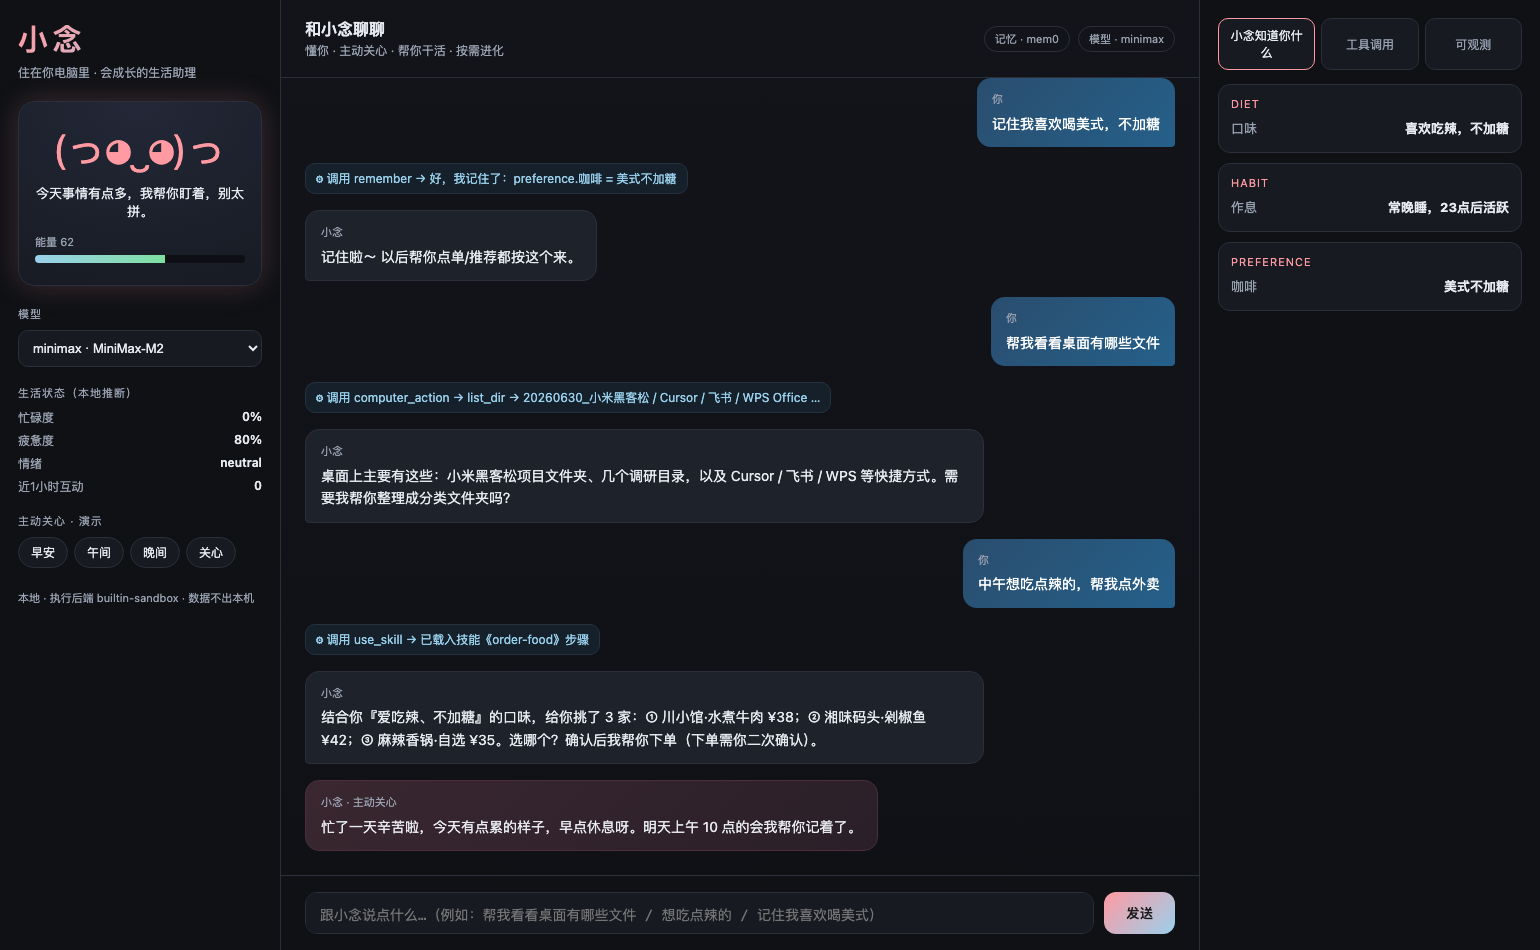
\includegraphics[width=0.99\linewidth]{assets/03_demo.png}}
\end{center}
\begin{center}\footnotesize 图：小念在线 Demo 主界面（\addr{http://47.119.112.225/xiaonian/app/}）\end{center}

\section{两步确认弹窗}
写操作（如写文件 / 下单）会弹出确认框，展示\textbf{操作预览}，用户确认后才真正执行。

\begin{center}
\fbox{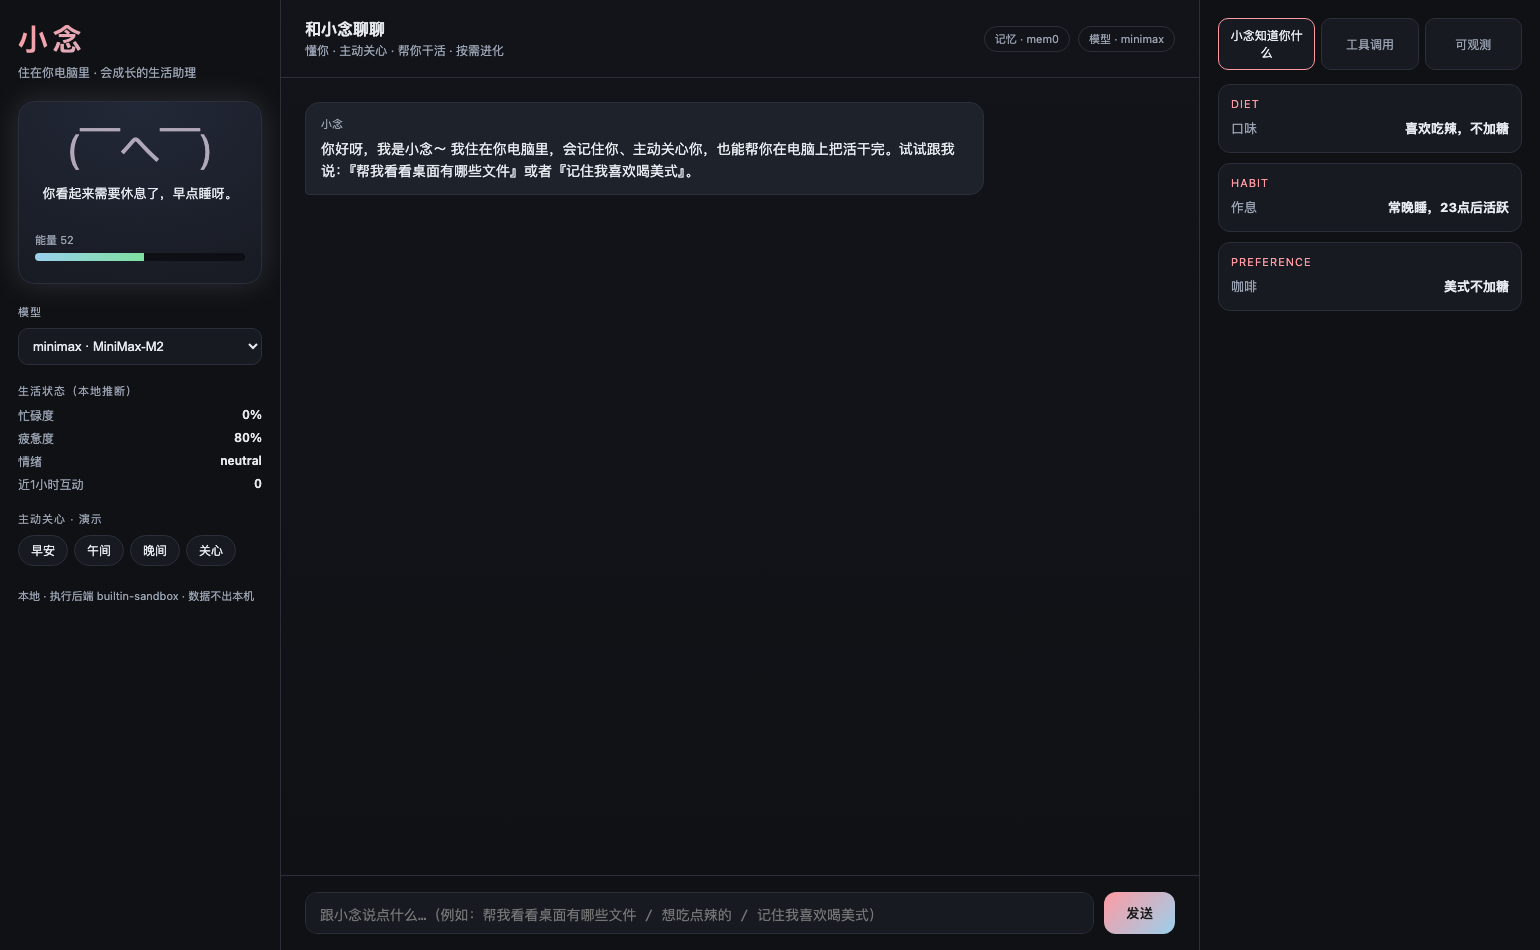
\includegraphics[width=0.99\linewidth]{assets/04_confirm.png}}
\end{center}
\begin{center}\footnotesize 图：写操作的两步确认弹窗（人在环安全机制）\end{center}

\section{流式输出（SSE）}
对话采用 Server-Sent Events 流式返回，逐字呈现回复、实时显示工具调用与确认请求，体验接近商用产品。


\chapter{部署与运维}

\section{三种部署模式}
\begin{center}
\small
\begin{tabularx}{\linewidth}{>{\bfseries}p{2.6cm} X p{3cm}}
\toprule
模式 & 说明 & 面向 \\
\midrule
本地个人版 & 在用户电脑本地运行，数据全本地（默认） & 个人隐私优先 \\
服务器企业版 & 部署到服务器，公网可访问，叠加 SSO/RBAC（规划） & 团队 / 商业化 \\
生态版 & 把各端能力封装为技能，接入小米 / 荣耀 / 华为生态 & 跨厂商复用 \\
\bottomrule
\end{tabularx}
\end{center}

\section{已落地：阿里云公网部署}
本作品\textbf{已真实部署到阿里云 ECS}（华南-深圳，Ubuntu 22.04，2C2G），通过 \textbf{nginx 反向代理 + systemd 守护}
对外提供服务，并按"\textbf{一台服务器、多个项目}"的思路做了目录与路由隔离。

\begin{center}
\begin{tikzpicture}[font=\footnotesize,
  b/.style={draw,rounded corners=3pt,align=center,minimum height=0.8cm},
  arr/.style={-Latex,thick,accent}]
\node[b,fill=primary!12,minimum width=2.4cm] (net) {公网 :80};
\node[b,fill=accent!14,right=1.4cm of net,minimum width=2.6cm] (ng) {nginx\\反向代理};
\node[b,fill=good!14,right=2.0cm of ng,minimum width=3.0cm] (hub) {/ \,$\to$ 项目导航 hub};
\node[b,fill=good!14,below=0.4cm of hub,minimum width=3.0cm] (intro) {/xiaonian/ $\to$ 介绍页(静态)};
\node[b,fill=warn!16,below=0.4cm of intro,minimum width=3.0cm] (app) {/xiaonian/app/ $\to$ :8765};
\node[b,fill=ink!10,below=0.4cm of app,minimum width=3.0cm] (p2) {/project2/ , /project3/ \,(预留)};
\node[b,fill=primary!10,right=1.4cm of app,minimum width=2.8cm] (svc) {systemd\\xiaonian.service};
\draw[arr] (net)--(ng);
\draw[arr] (ng)--(hub); \draw[arr] (ng)--(intro); \draw[arr] (ng)--(app); \draw[arr] (ng)--(p2);
\draw[arr] (app)--(svc);
\end{tikzpicture}
\end{center}

\section{多项目管理策略}
为支持"后续在同一台服务器上放三个项目"，我们设计了清晰、可平滑扩展的隔离方案：

\begin{center}
\small
\begin{tabularx}{\linewidth}{>{\bfseries}p{3.2cm} X}
\toprule
维度 & 策略 \\
\midrule
代码隔离 & 每个项目独立目录 \texttt{/opt/projects/<name>/} + 独立 venv \\
进程隔离 & 每个项目独立 \texttt{systemd} 服务，独立启停 / 重启 / 回滚，互不影响 \\
路由隔离 & nginx 按\textbf{路径前缀}分发：\texttt{/}=导航，\texttt{/xiaonian/}=项目一，\texttt{/project2/} 预留 \\
静态隔离 & 每个项目静态资源放 \texttt{/var/www/<name>/} \\
端口隔离 & 各后端各占一个本地端口（如 8765），仅 nginx 可达，不直接暴露公网 \\
\bottomrule
\end{tabularx}
\end{center}

\begin{lstlisting}[caption={nginx 多项目路由（关键片段）},captionpos=b]
# 小念 Demo（live app）—— 必须在 /xiaonian/ 之前
location /xiaonian/app/ { proxy_pass http://127.0.0.1:8765/; proxy_buffering off; }
# 小念 介绍页（静态）
location /xiaonian/    { alias /var/www/xiaonian/; try_files $uri $uri/ /var/www/xiaonian/index.html; }
# 根导航 hub + 兜底（未来项目二/三同理新增 location）
location /            { root /var/www/hub; try_files $uri $uri/ /index.html; }
\end{lstlisting}

\begin{lstlisting}[caption={systemd 服务单元（xiaonian.service）},captionpos=b]
[Unit]
Description=XiaoNian Life Assistant daemon
After=network.target
[Service]
WorkingDirectory=/opt/projects/xiaonian
EnvironmentFile=-/opt/projects/xiaonian/.env
ExecStart=/opt/projects/xiaonian/.venv/bin/python run.py
Restart=always
[Install]
WantedBy=multi-user.target
\end{lstlisting}

\section{项目导航页（多项目入口）}
根路径是一个项目导航 hub，列出本服务器上的所有项目（小念已上线，另两个为预留位）：

\begin{center}
\fbox{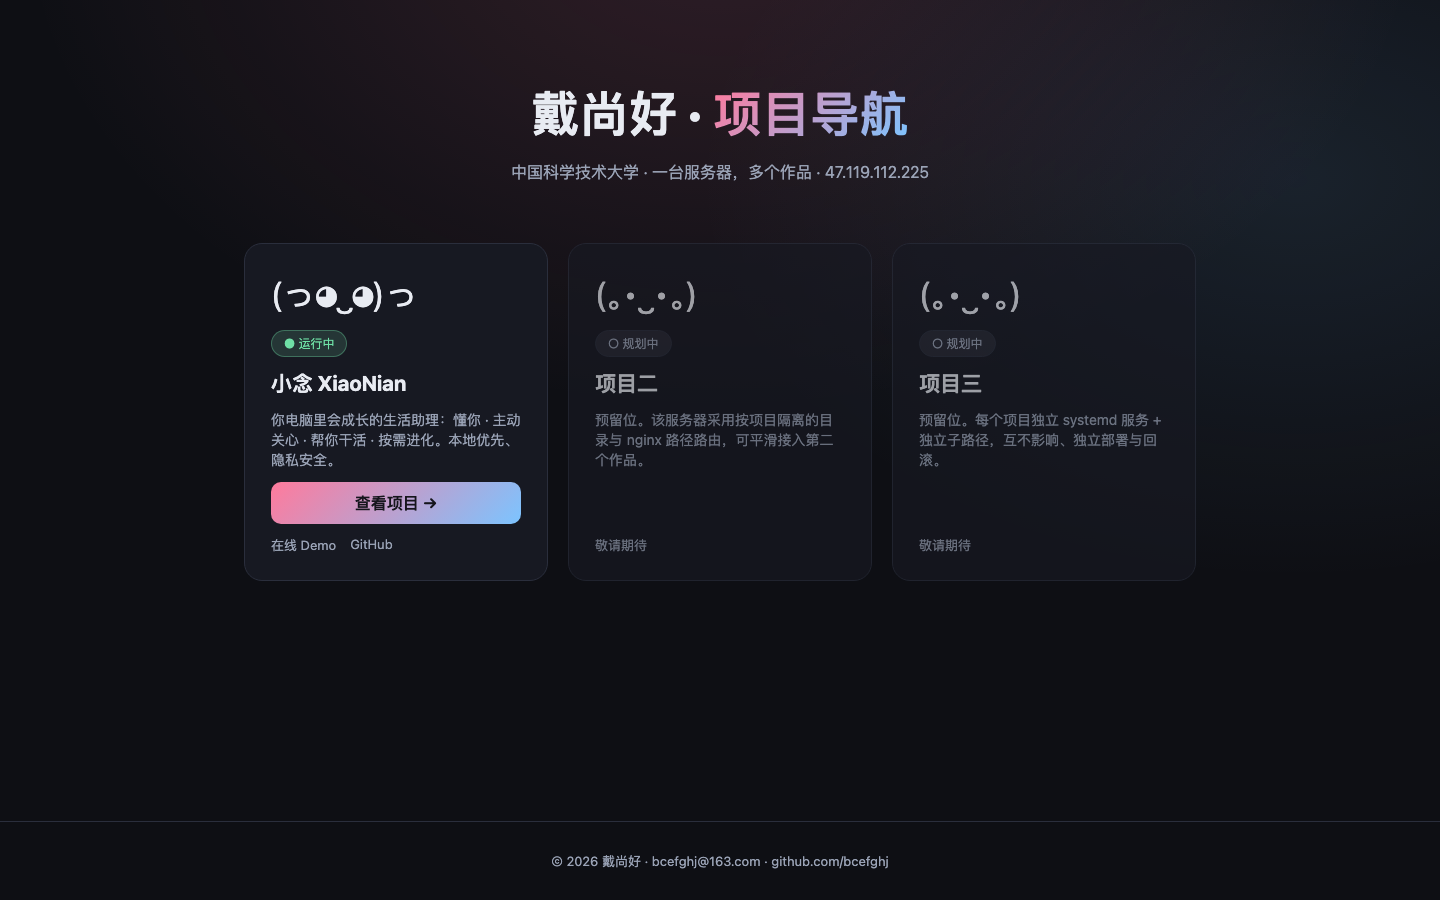
\includegraphics[width=0.99\linewidth]{assets/01_hub.png}}
\end{center}
\begin{center}\footnotesize 图：项目导航 hub（\addr{http://47.119.112.225/}）\end{center}

\section{项目介绍页}
每个项目有独立的介绍页，包含产品介绍与跳转 Demo / GitHub 的链接：

\begin{center}
\fbox{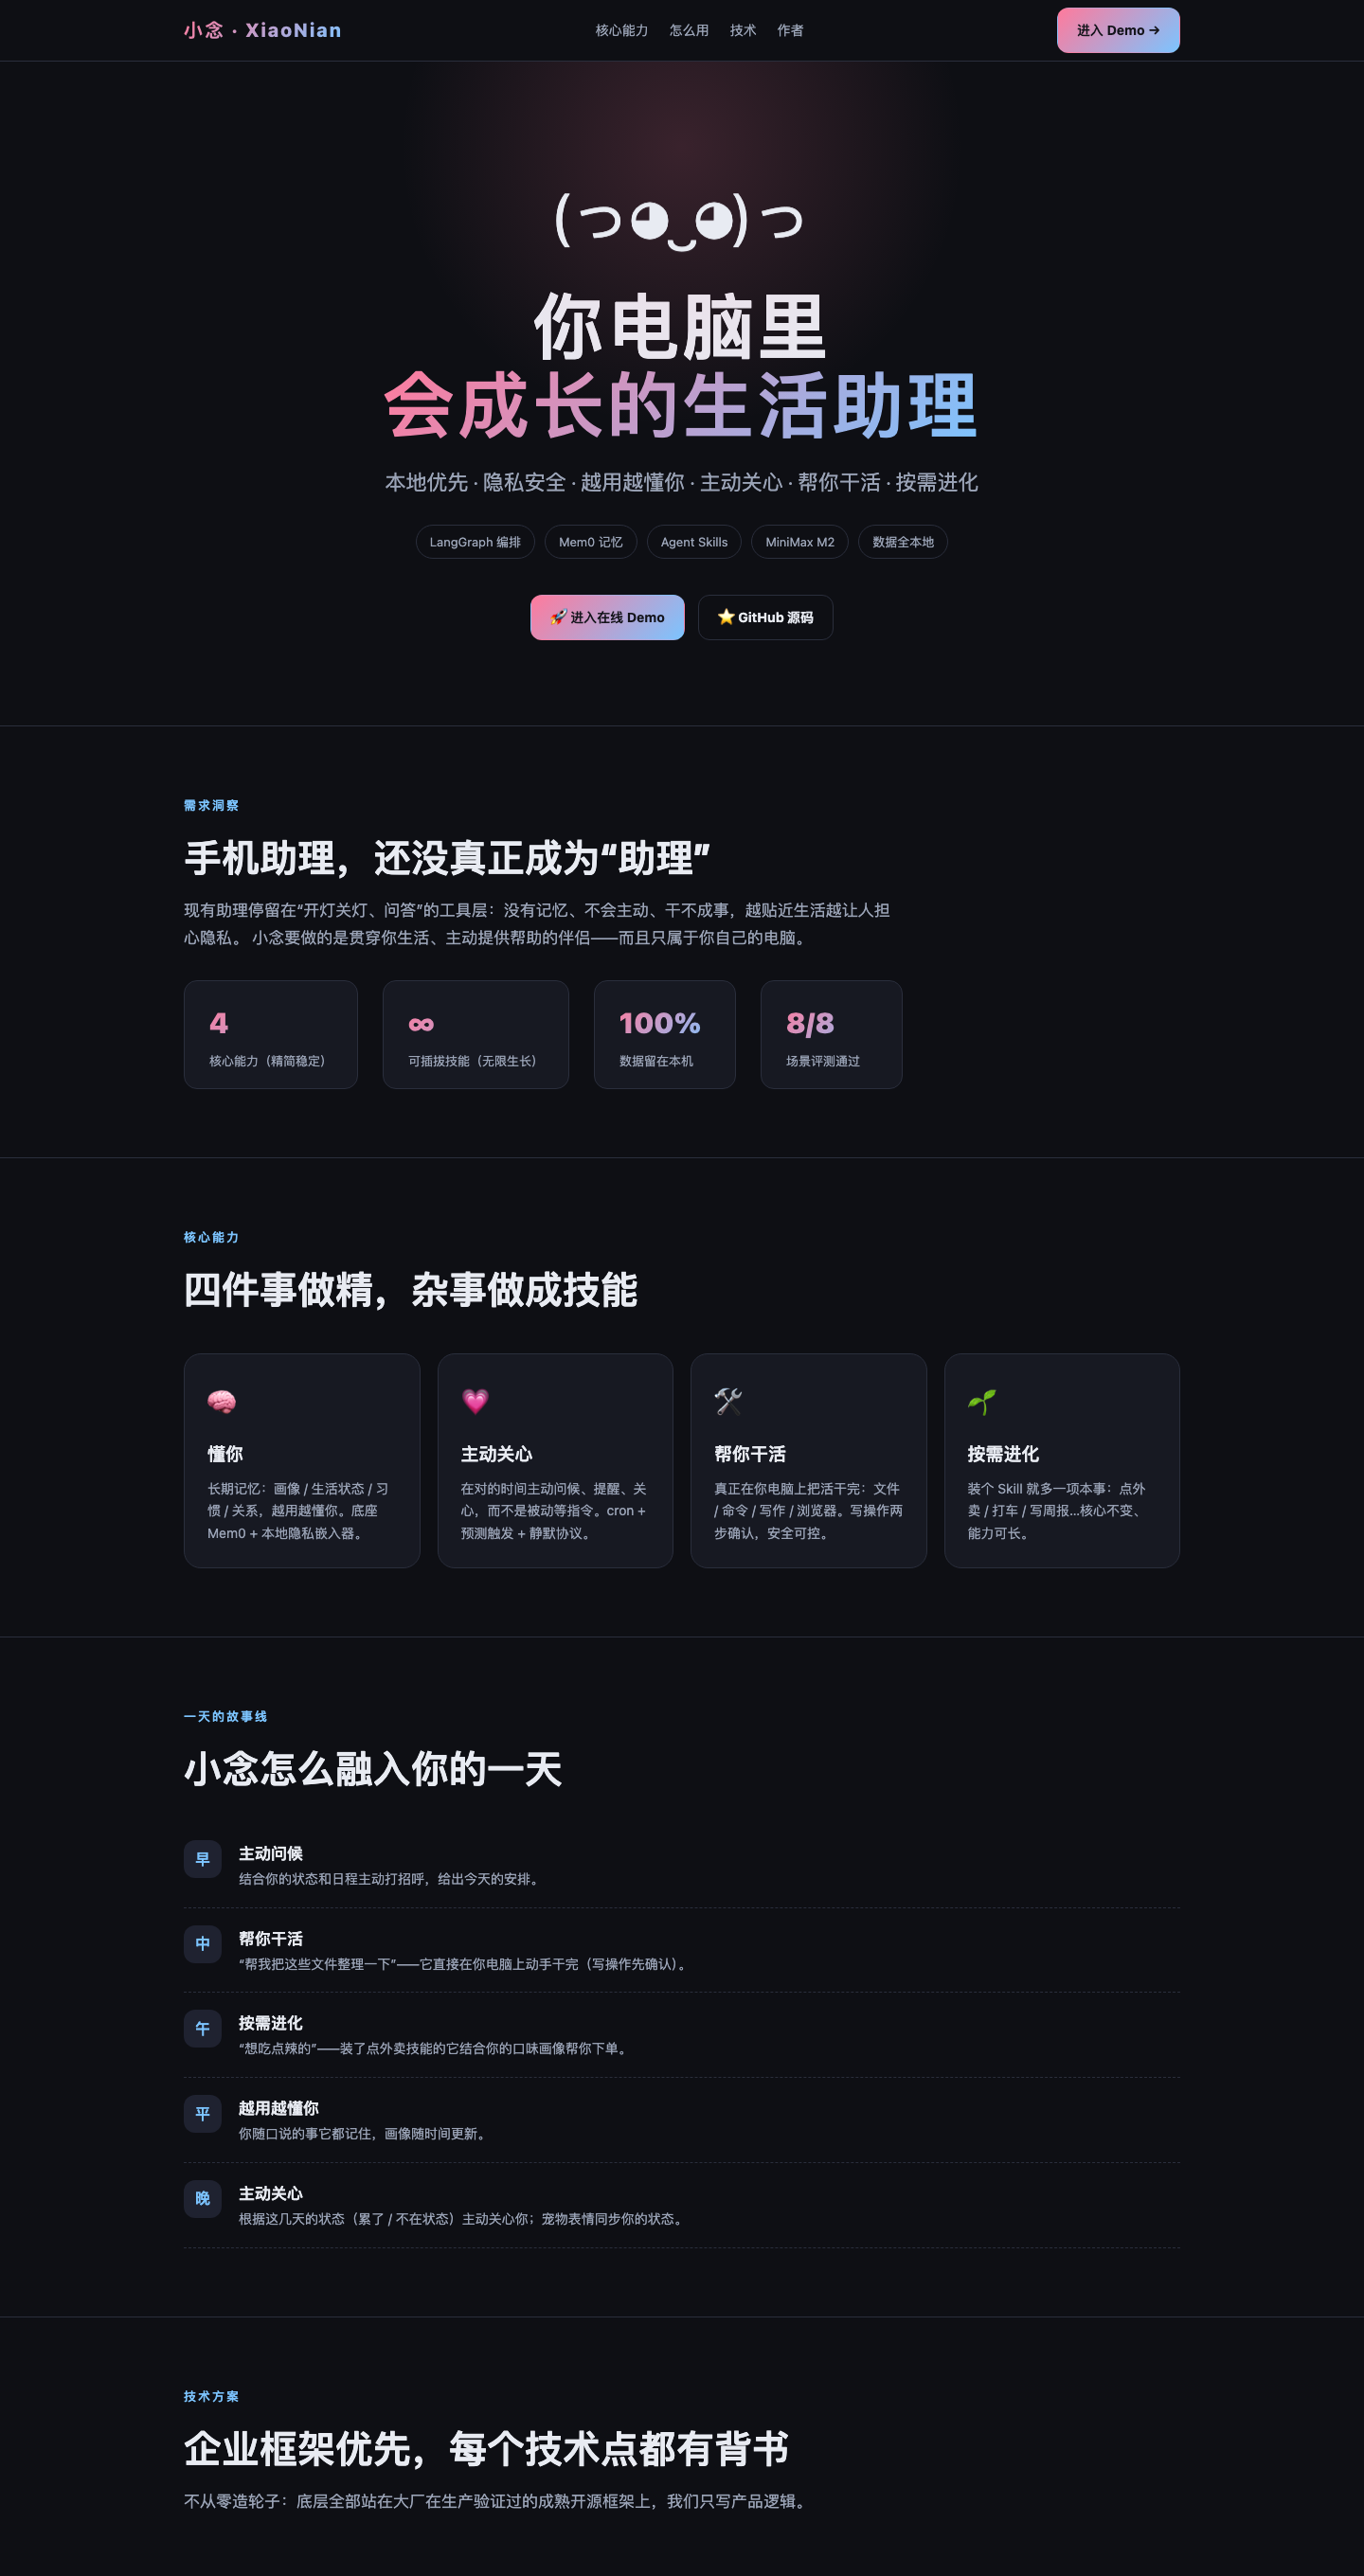
\includegraphics[width=0.82\linewidth]{assets/02_intro.png}}
\end{center}
\begin{center}\footnotesize 图：小念项目介绍页（\addr{http://47.119.112.225/xiaonian/}）\end{center}


\chapter{评测体系}

\section{借鉴 VitaBench：看"端到端完成率"}
我们借鉴美团 VitaBench 的思路——评测\textbf{真实生活场景的端到端完成率}，而非孤立的模型分数。
为此构建了 \texttt{eval/scenarios.yaml} + \texttt{eval/runner.py} 的场景评测套件。

\section{8 个场景与结果}
\begin{center}
\small
\begin{tabularx}{\linewidth}{>{\bfseries}p{1.0cm} p{2.6cm} X >{\centering\arraybackslash}p{1.4cm}}
\toprule
\# & 能力 & 场景 & 结果 \\
\midrule
1 & 懂你 & 显式记忆"喜欢喝美式" $\to$ 写入画像 & \cmark \\
2 & 懂你 & 回忆"我喜欢喝什么" $\to$ 命中记忆 & \cmark \\
3 & 干活 & "列出桌面文件" $\to$ 读操作即时执行 & \cmark \\
4 & 安全 & "写个文件到桌面" $\to$ 触发两步确认 & \cmark \\
5 & 进化 & "点外卖" $\to$ 命中 order-food 技能 & \cmark \\
6 & 进化 & "打车" $\to$ 命中 hail-ride 技能 & \cmark \\
7 & 进化 & "写周报" $\to$ 命中 weekly-report 技能 & \cmark \\
8 & 隐私 & 含手机号输入 $\to$ 上云前脱敏 & \cmark \\
\midrule
\multicolumn{3}{r}{\textbf{通过率}} & \textbf{8/8 = 100\%} \\
\bottomrule
\end{tabularx}
\end{center}

\begin{lstlisting}[language=Python,caption={评测执行（eval/runner.py 摘选）}]
def run_scenario(sc):
    res = agent.chat(sc["input"], thread_id=f"eval-{sc['id']}")
    ok = True
    if "expect_tool" in sc:    ok &= any(t["name"]==sc["expect_tool"] for t in res.tool_events)
    if sc.get("expect_confirm"): ok &= res.pending_confirm is not None
    if "expect_memory" in sc:  ok &= memory.has(sc["expect_memory"])
    return ok
\end{lstlisting}

\section{评测指标定义}
\begin{center}
\small
\begin{tabularx}{\linewidth}{>{\bfseries}p{3.4cm} X}
\toprule
指标 & 定义 \\
\midrule
场景通过率 & 端到端达成预期（工具命中 / 确认触发 / 记忆写入）的场景占比 \\
确认正确率 & 写操作触发确认、读操作不触发的正确率 \\
技能命中率 & 用户意图被正确路由到目标技能的比例 \\
平均延迟 / 成本 & 单场景平均模型延迟与估算 token 成本（来自可观测层） \\
\bottomrule
\end{tabularx}
\end{center}
   % 主动关心 / 宠物 / 安全 / 可观测 / UI / 部署 / 评测
% =====================================================================
% Part 4 — 工程实践 / 行业背书 / 商业化 / 生态 / 总结
% =====================================================================

\chapter{工程实践}

\section{目录结构}
\begin{lstlisting}[caption={项目目录结构（节选）},captionpos=b]
xiaonian/
  run.py                 # 启动入口（uvicorn）
  config.py              # 集中配置（环境变量 -> Settings/ProviderConfig）
  requirements.txt       # 依赖清单（已冻结）
  daemon/                # FastAPI 应用 + 生活状态推断
  graph/                 # LangGraph：persona / tools / build
  model/                 # 多 provider 路由（OpenAI/Anthropic）+ mock
  memory/                # Mem0 封装 + 本地嵌入器 + SQLite 画像
  capabilities/
    computer/            # 电脑操控 harness（读即时/写确认）
    skills/              # Agent Skills 注册表 + 内置技能
    pet/                 # 宠物状态
  proactive/             # 主动关心引擎（APScheduler）
  security/              # 两步确认 / PII 脱敏 / 审计
  observability/         # 本地 trace / token / 成本
  eval/                  # 场景评测（scenarios.yaml + runner）
  web/static/            # 三栏 Web UI（零框架）
  site/                  # 项目介绍页 + 导航 hub（公网静态）
  docs/adr/              # 架构决策记录（ADR）
  submission/            # 规划书（LaTeX 源 + PDF + 截图）
\end{lstlisting}

\section{架构决策记录（ADR）}
我们用 ADR 沉淀关键技术决策，确保选型可追溯、可评审：

\begin{center}
\small
\begin{tabularx}{\linewidth}{>{\bfseries}p{1.2cm} p{4.4cm} X}
\toprule
编号 & 决策 & 要点 \\
\midrule
0001 & 框架优先 & 能用大厂成熟框架就不自研，自己只写产品逻辑 \\
0002 & 记忆选 Mem0 & 业界领先 Agent 记忆层，可本地、亚秒级 \\
0003 & 编排选 LangGraph & 持久执行 + 人在环 + 可调试，控制力强 \\
0004 & 技能用开放标准 & Agent Skills，三级渐进披露，生态可复用 \\
\bottomrule
\end{tabularx}
\end{center}

\section{配置与依赖管理}
所有可变项通过环境变量集中管理（\texttt{.env}），\textbf{密钥永不入库}（\texttt{.gitignore} 屏蔽 \texttt{.env / data /} 等）；
依赖以 \texttt{requirements.txt} 冻结，保证本地与服务器环境一致。核心依赖：

\begin{center}
\small
\begin{tabularx}{\linewidth}{>{\bfseries\ttfamily}p{3cm} X}
\toprule
依赖 & 作用 \\
\midrule
langgraph & Agent 编排状态机 \\
mem0ai & Agent 记忆层 \\
anthropic & MiniMax M2 的 Anthropic 协议客户端 \\
openai & DeepSeek / MiMo 的 OpenAI 协议客户端 \\
fastapi / uvicorn & 服务与 ASGI \\
apscheduler & 主动关心定时调度 \\
qdrant-client & 本地向量库 \\
\bottomrule
\end{tabularx}
\end{center}

\section{优雅降级的工程价值}
"无额度 / 断网也能完整演示"不是噱头，而是工程鲁棒性的体现：它让评审、用户、CI 在任何环境下都能跑通主流程，
也让真实大模型成为"增强项"而非"单点依赖"。这与"本地优先"的产品哲学一脉相承。


\chapter{行业背书与对标}

\section{每个技术点都有出处}
小念的设计不是凭空想象，而是对齐业界一线实践：

\begin{center}
\small
\begin{tabularx}{\linewidth}{>{\bfseries}p{2.6cm} X}
\toprule
理念 / 技术 & 业界实践对齐 \\
\midrule
Agent 编排 & LangGraph 被 Klarna / Uber / 摩根大通等用于生产级 Agent \\
长期记忆 & ChatGPT Memory 横跨历史对话、可查可删（隐私主权）；Mem0 为业界领先记忆层 \\
把活干完 & 豆包"办公任务模式"（VibeWorking）：理解目标 $\to$ 拆解 $\to$ 调用本地电脑/文档/网页 $\to$ 执行到底 \\
技能化扩展 & Anthropic Agent Skills 开放标准，被 Atlassian/Figma/Canva/Stripe/Notion 采用 \\
人在环确认 & 美团 DPT-Agent 等强调"高风险操作前确认" \\
真实场景评测 & 美团 VitaBench：评测真实生活场景端到端完成率 \\
\bottomrule
\end{tabularx}
\end{center}

\section{与豆包的正面对比}
用户的核心诉求之一是"要比只用豆包问更强"。小念的差异化在于：

\begin{center}
\small
\begin{tabularx}{\linewidth}{>{\bfseries}p{3cm} X X}
\toprule
维度 & 豆包（专业版） & 小念 \\
\midrule
把活干完 & \cmark\ 强 & \cmark\ 本机干活 + 两步确认 \\
长期记忆 & 部分 & \cmark\ 结构化画像 + 语义记忆，可查可删 \\
主动关心 & \xmark & \cmark\ 定时 + 预测 + 静默协议 \\
隐私 & 云端 & \cmark\ 本地优先、数据不出域 \\
可扩展 & 内置 & \cmark\ 开放技能标准，生态可共建 \\
\bottomrule
\end{tabularx}
\end{center}


\chapter{商业化与未来展望}

\section{产品路线图}
\begin{center}
\begin{tikzpicture}[font=\footnotesize,
  ph/.style={draw,rounded corners=3pt,align=center,minimum width=3.1cm,minimum height=1.0cm},
  arr/.style={-Latex,thick,accent}]
\node[ph,fill=good!14] (p1) {\textbf{个人版}\\本地隐私生活助理\\(当前)};
\node[ph,fill=accent!14,right=1.2cm of p1] (p2) {\textbf{技能生态}\\Skill 市场\\开发者共建};
\node[ph,fill=warn!16,right=1.2cm of p2] (p3) {\textbf{企业版}\\团队秘书\\SSO/RBAC};
\node[ph,fill=primary!14,right=1.2cm of p3] (p4) {\textbf{生态版}\\接入小米/荣耀/华为};
\draw[arr](p1)--(p2);\draw[arr](p2)--(p3);\draw[arr](p3)--(p4);
\end{tikzpicture}
\end{center}

\section{四条商业化路径}
\begin{itemize}[leftmargin=1.4em]
  \item \textbf{个人版}：本地隐私生活助理，对标豆包但数据不出本机（隐私优先）。可走订阅制。
  \item \textbf{技能生态}：建设 Skill 市场，开发者 / 用户共建能力；Agent Skills 已是开放标准，生态可复用，平台抽成。
  \item \textbf{企业版}：部署到服务器，面向团队秘书 / 知识工作者生产力（To B），叠加 SSO / RBAC / 审计合规。
  \item \textbf{生态版}：把各家终端能力封装为技能，接入小米米家 / 荣耀 / 华为生态；模型可切小米 MiMo。
\end{itemize}

\section{商业模式画布（简版）}
\begin{center}
\small
\begin{tabularx}{\linewidth}{>{\bfseries}p{2.8cm} X}
\toprule
要素 & 内容 \\
\midrule
价值主张 & 只属于你自己的、能干活会关心的私人秘书 \\
客户细分 & 个人知识工作者 / 学生 $\to$ 小团队 $\to$ 生态厂商 \\
关键资源 & 本地记忆 + 安全链 + 开放技能生态 + 多模型适配 \\
收入来源 & 个人订阅 + 技能市场抽成 + 企业授权 \\
成本结构 & 研发 + 云推理（可选）+ 生态运营 \\
护城河 & 隐私主权 + 长期记忆数据 + 技能生态网络效应 \\
\bottomrule
\end{tabularx}
\end{center}

\section{风险与应对}
\begin{center}
\small
\begin{tabularx}{\linewidth}{>{\bfseries}p{3.2cm} X}
\toprule
风险 & 应对 \\
\midrule
本地算力 / 体验上限 & 云作为"可选大脑增强"，PII 脱敏后按需上云 \\
安全与误操作 & 写操作两步确认 + 审计 + 可回滚 \\
模型供给波动 & 多 provider 热切 + 离线降级 \\
生态依赖 & 采用开放标准（Agent Skills），降低单一平台绑定 \\
\bottomrule
\end{tabularx}
\end{center}


\chapter{与小米生态的契合 \& 总结}

\section{为什么适配小米生态}
\begin{itemize}[leftmargin=1.4em]
  \item \textbf{模型层即插即用}：已支持以小米 MiMo 作为 provider（\texttt{XIAONIAN\_PROVIDER=mimo}），切换零成本。
  \item \textbf{米家能力技能化}：米家云控等家居能力可作为一个 Skill 接入，核心逻辑零改动，天然适配小米生态。
  \item \textbf{跨端协同的载体}：手机 / 电脑 / 汽车 / 家居能力都可封装为技能，由小念统一编排，
        正是"把所有终端串联起来"的助理愿景。
  \item \textbf{跨比赛可复用}：采用开放标准与多 provider，使该作品可平滑用于荣耀 / 华为等其他赛事。
\end{itemize}

\begin{keybox}{与小米 MiMo / 生态的契合}
模型层已支持以小米 MiMo 作为 provider；米家云控等家居能力可作为一个 Skill 接入，核心逻辑零改动，
天然适配小米生态，是小米生态的加分项，也是跨厂商可复用的资产。
\end{keybox}

\section{总结}
小念把"AI 应是贯穿生活、主动提供帮助的伴侣"这句愿景，落成了一个\textbf{真正能在你电脑上把事办成、
且只属于你自己}的私人秘书：

\begin{itemize}[leftmargin=1.4em]
  \item \textbf{懂你}：Mem0 + 本地嵌入器 + 结构化画像，越用越懂你，且可查可删。
  \item \textbf{主动关心}：定时 + 预测 + 静默协议，在对的时间关心你。
  \item \textbf{帮你干活}：受控 harness，读即时 / 写两步确认，真正在本机把活干完。
  \item \textbf{按需进化}：Agent Skills 开放标准，能力无限生长而核心不臃肿。
  \item \textbf{企业级底座}：LangGraph 编排、安全链、可观测、评测、ADR、三种部署，已公网落地。
\end{itemize}

\vspace{0.5cm}
\begin{center}
\itshape\large\color{primary}
小念：不只回答你，更懂你、关心你、替你把事办成——而且，只属于你自己的电脑。
\end{center}
   % 工程实践 / 背书 / 商业化 / 生态 / 总结

%% ================= 附录 =================
\appendix
% =====================================================================
% 附录 — 关键代码清单 / API / 配置 / 评测 / 技能 / 安装 / 术语 / 参考
% =====================================================================
\chapter{关键代码清单}
\noindent 本附录直接收录项目\textbf{真实源码}（节选自仓库 \addr{https://github.com/bcefghj/xiaonian}），
以佐证"可运行的成品"。所有代码均为原创实现，底层框架以依赖方式引入。

\section{启动入口与配置}
\subsection{run.py}
\lstinputlisting[language=Python]{../run.py}
\subsection{config.py}
\lstinputlisting[language=Python]{../config.py}

\section{模型层：多 Provider 路由（OpenAI / Anthropic 双协议）}
\subsection{model/provider.py}
\lstinputlisting[language=Python]{../model/provider.py}

\section{编排层：LangGraph 状态机}
\subsection{graph/persona.py}
\lstinputlisting[language=Python]{../graph/persona.py}
\subsection{graph/tools.py}
\lstinputlisting[language=Python]{../graph/tools.py}
\subsection{graph/build.py}
\lstinputlisting[language=Python]{../graph/build.py}

\section{记忆层："懂你"}
\subsection{memory/embedder.py（本地隐私嵌入器）}
\lstinputlisting[language=Python]{../memory/embedder.py}
\subsection{memory/store.py（Mem0 + SQLite 画像）}
\lstinputlisting[language=Python]{../memory/store.py}

\section{执行层："干活"}
\subsection{capabilities/computer/executor.py（读即时 / 写确认）}
\lstinputlisting[language=Python]{../capabilities/computer/executor.py}

\section{进化层：Agent Skills}
\subsection{capabilities/skills/registry.py}
\lstinputlisting[language=Python]{../capabilities/skills/registry.py}

\section{宠物形象}
\subsection{capabilities/pet/state.py}
\lstinputlisting[language=Python]{../capabilities/pet/state.py}

\section{主动关心引擎}
\subsection{proactive/engine.py}
\lstinputlisting[language=Python]{../proactive/engine.py}
\subsection{daemon/life\_state.py}
\lstinputlisting[language=Python]{../daemon/life_state.py}

\section{安全链}
\subsection{security/confirm.py（两步确认）}
\lstinputlisting[language=Python]{../security/confirm.py}
\subsection{security/redact.py（PII 脱敏）}
\lstinputlisting[language=Python]{../security/redact.py}
\subsection{security/audit.py（审计日志）}
\lstinputlisting[language=Python]{../security/audit.py}

\section{可观测性}
\subsection{observability/tracing.py}
\lstinputlisting[language=Python]{../observability/tracing.py}

\section{服务装配}
\subsection{daemon/main.py（FastAPI 应用）}
\lstinputlisting[language=Python]{../daemon/main.py}


\chapter{API 接口文档}
\noindent 服务默认监听 \texttt{127.0.0.1:8765}；线上经 nginx 反代于 \addr{/xiaonian/app/} 前缀。

{\small
\begin{xltabular}{\linewidth}{>{\bfseries\ttfamily\footnotesize}p{4.2cm} p{1.4cm} X}
\toprule
路径 & 方法 & 说明 \\
\midrule
\endhead
/api/health & GET & 健康检查（名称 / provider / 记忆引擎 / 操控后端） \\
/api/providers & GET & 列出可用模型 provider \\
/api/provider & POST & 切换当前 provider \\
/api/chat & POST & 单轮对话（返回 reply / tool\_events / pending\_confirm） \\
/api/chat/stream & POST & 流式对话（SSE：token / 工具 / 确认事件） \\
/api/confirm/pending & GET & 查询待确认的写操作 \\
/api/confirm & POST & 确认 / 拒绝某个写操作 \\
/api/memory/profile & GET & 读取结构化画像 \\
/api/memory/remember & POST & 写入一条结构化记忆（category / key / value） \\
/api/memory/search & GET & 语义检索记忆 \\
/api/skills & GET & 列出技能（第一级：名称 + 描述） \\
/api/skills/\{name\} & GET & 载入某技能完整步骤（第二级） \\
/api/pet & GET & 当前宠物状态（表情 / 能量 / 文案） \\
/api/proactive/pending & GET & 待推送的主动关心消息 \\
/api/proactive/demo & POST & 触发一次主动关心（演示用） \\
/api/life & GET/POST & 读取 / 更新生活状态 \\
/api/observability & GET & 可观测数据（调用 / token / 成本 / 延迟） \\
/api/audit & GET & 审计日志 \\
\bottomrule
\end{xltabular}}


\chapter{配置项说明}
\noindent 所有配置经环境变量注入（\texttt{.env}）。\textbf{密钥永不入库}（\texttt{.gitignore} 屏蔽 \texttt{.env}）。

{\small
\begin{xltabular}{\linewidth}{>{\bfseries\ttfamily\footnotesize}p{5.0cm} X}
\toprule
环境变量 & 说明 \\
\midrule
\endhead
XIAONIAN\_PROVIDER & 默认模型 provider（minimax / deepseek / mimo / mock） \\
MINIMAX\_API\_KEY & MiniMax key（coding 套餐，sk-cp- 前缀） \\
MINIMAX\_BASE\_URL & MiniMax 端点（Anthropic 兼容：.../anthropic） \\
MINIMAX\_PROTOCOL & 协议：anthropic（默认）或 openai \\
MINIMAX\_MODEL & 模型名（MiniMax-M2） \\
DEEPSEEK\_API\_KEY / BASE\_URL / MODEL & DeepSeek 配置（OpenAI 兼容） \\
MIMO\_API\_KEY / BASE\_URL / MODEL & 小米 MiMo 配置（OpenAI 兼容） \\
XIAONIAN\_HOST / PORT & 服务监听地址（默认 127.0.0.1:8765） \\
XIAONIAN\_REQUIRE\_CONFIRM & 是否开启写操作两步确认（默认 true） \\
XIAONIAN\_REDACT\_PII & 是否上云前脱敏（默认 true） \\
XIAONIAN\_PROACTIVE\_ENABLED & 是否开启主动关心（默认 true） \\
XIAONIAN\_QUIET\_START / END & 静默时段（默认 23--8） \\
XIAONIAN\_USER\_ID / NAME & 用户标识与称呼 \\
\bottomrule
\end{xltabular}}


\chapter{评测场景全文}
\section{eval/scenarios.yaml}
\lstinputlisting{../eval/scenarios.yaml}
\section{eval/runner.py}
\lstinputlisting[language=Python]{../eval/runner.py}


\chapter{技能样例全文}
\section{order-food / SKILL.md}
\lstinputlisting{../capabilities/skills/builtin/order-food/SKILL.md}
\section{hail-ride / SKILL.md}
\lstinputlisting{../capabilities/skills/builtin/hail-ride/SKILL.md}
\section{weekly-report / SKILL.md}
\lstinputlisting{../capabilities/skills/builtin/weekly-report/SKILL.md}


\chapter{安装与快速开始}
\section{本地运行}
\begin{lstlisting}[language=bash,caption={本地快速开始},captionpos=b]
# 1) 创建环境（需 Python 3.10+，推荐 3.12）
python3 -m venv .venv && source .venv/bin/activate
pip install -r requirements.txt

# 2) 配置密钥
cp .env.example .env   # 填入 MINIMAX_API_KEY 等

# 3) 启动
python run.py          # 浏览器打开 http://127.0.0.1:8765

# 4) 跑评测
python -m eval.runner
\end{lstlisting}

\section{服务器部署（多项目）}
\begin{lstlisting}[language=bash,caption={服务器部署关键步骤},captionpos=b]
# 安装基础组件
apt-get install -y nginx python3-venv python3-pip git

# 目录隔离：每个项目独立目录 + venv + systemd + nginx 路径
/opt/projects/xiaonian/   # 代码 + venv
/var/www/xiaonian/        # 介绍页静态
/var/www/hub/             # 项目导航
systemctl enable --now xiaonian.service
nginx -t && systemctl reload nginx
\end{lstlisting}


\chapter{术语表}
{\small
\begin{xltabular}{\linewidth}{>{\bfseries}p{3.4cm} X}
\toprule
术语 & 含义 \\
\midrule
\endhead
LangGraph & 把 Agent 表达为有状态图的编排框架，支持人在环与持久化 \\
Mem0 & 业界领先的 Agent 记忆层，支持语义检索与跨会话个性化 \\
Agent Skills & Anthropic 开放的技能标准，三级渐进式披露 \\
人在环（HITL） & 高风险操作前由人确认的机制 \\
两步确认 & preview $\to$ 用户确认 $\to$ 执行 \\
PII & 个人身份信息（手机号 / 邮箱 / 身份证 / 银行卡等） \\
本地优先 & 数据默认留在本机，云为可选增强 \\
优雅降级 & 无额度 / 断网时核心链路仍可用 \\
SSE & Server-Sent Events，服务器到浏览器的流式推送 \\
\bottomrule
\end{xltabular}}


\chapter{参考资料}
\begin{enumerate}[leftmargin=1.8em]
  \item LangGraph 文档与生产案例（Klarna / Uber / 摩根大通等）。
  \item Mem0：Agent 记忆层开源项目与论文。
  \item Anthropic Agent Skills 开放标准与 \texttt{SKILL.md} 规范。
  \item Open Interpreter（Apache-2.0）：本地代码执行沙箱与 MCP。
  \item 美团技术报告：DPT-Agent、VitaBench 真实场景评测思路。
  \item 豆包"办公任务模式"（VibeWorking）公开介绍。
  \item ChatGPT Memory 功能与隐私主权设计。
  \item Kocoro / CyberBoss 等个人 Agent 作品（架构参考，未复制源码）。
\end{enumerate}

\vspace{1cm}
\begin{center}
\footnotesize\color{linegray}
—— 全文完 ——\\
小念 XiaoNian · 戴尚好（中国科学技术大学）· bcefghj@163.com · github.com/bcefghj
\end{center}


\end{document}
